\chapter{Introduction}
\label{introduction}
A finite automaton (FA) is a model of computation with applications in different branches of computer science, e.g., compiler design, formal verification, 
the design of digital circuits or natural language processing. In formal verification alone are its uses abundant, 
for example in model checking of safety temporal properties \cite{principles}, abstract regular model checking \cite{armc}, static analysis \cite{metal}, 
or decision procedures of some logics, such as Presburger arithmetic or weak 
monadic second-order theory of one successor (WS1S) \cite{mona}.

Many of the mentioned applications need to perform certain expensive operations on FA, such as checking universality of an FA (i.e., checking whether it
accepts any word over a given alphabet), or checking language inclusion of a pair of FA (i.e., testing whether the language of one FA is a subset of the language
of the other FA). The classical (so called \emph{textbook}) approach is based on \emph{complementation} of the language of one of the FA. 
Complementation is easy for 
\emph{deterministic} FA (DFA)---just swapping accepting and non-accepting states---but a hard problem for \emph{nondeterministic} FA (NFA), which need 
to be determinised first (this may lead to an exponential explosion in the number of the states of the automaton). 
Both operations of checking of universality and language inclusion over NFA are PSPACE-complete problems \cite{cav06}.

Recently, there has been a considerable advance in techniques for dealing with these two problems. The new techniques are either based on the so-called 
\emph{antichains} \cite{cav06,tacas10} or the so-called \emph{bisimulation up to congruence} \cite{popl13}. 
In general, those techniques do not need an explicit construction of the complement
automaton. They only construct a sub-automaton which is sufficient for either proving that the universality or inclusion hold, or finding a counterexample.

Unfortunately, there is currently no efficient implementation of a general NFA library that would use the state-of-the-art algorithms for the mentioned
operations on automata. The
closest implementation is VATA \cite{libvata}, a general library for nondeterministic finite \emph{tree} automata, which can be used even for NFA (being modelled 
as unary tree automata) but not with the optimal performance given by its overhead that comes with the ability to handle much richer structures. 
 
The goal of this work is two-fold: (i) extending VATA with an NFA module implementing basic operations on NFA, such as union, intersection, or 
checking language inclusion, and (ii) an efficient design and implementation of operations for checking language inclusion of NFA using 
bisimulation up to congruence (which is missing in VATA for tree automata).

After this introduction, Chapter \ref{teorie} of this text describes the theoretical background. 
Chapter \ref{chapInclusion} provides a description of recently proposed 
efficient approaches to language inclusion testing and their optimization.
A list of the existing libraries for finite automata manipulation is given in Chapter \ref{libraries}. The same chapter
provides a brief description of the VATA library.
The design of the new module of the VATA library and algorithms used therein are described in Chapter \ref{design}. 
The implementation optimization of the algorithms for language inclusion checking and issues of other implementation is discussed in Chapter \ref{implementation}.
The evaluation of the optimized algorithms for the inclusion checking is in Chapter \ref{eval}. Chapter \ref{concl} summaries the thesis and gives directions for
future work.

\chapter{Preliminaries}
This chapter contains theoretical foundations of the thesis. No proofs are given but they can be found in the referenced literature \cite{kozen,ullman}. 
First, languages will be defined, then finite automata and their context and regular languages and their closure properties will follow. 
\label{teorie}

\section{Languages}
We call a finite set of symbols $\Sigma$ an \emph{alphabet}. A~\emph{word} $w$ over $\Sigma$ of \emph{length} $n$ is a finite sequence of symbols 
$w=a_1\cdots a_n$, where $\forall 1 \leq i \leq n\ . \ a_i \in \Sigma$. An \emph{empty word} is denoted as $\epsilon \not\in\Sigma$ and its length is $0$. 
We define \emph{concatenation} as an associative binary operation on words over $\Sigma$ represented by the symbol $\cdot$ such that for two words 
$u=a_1\cdots a_n$
and $v=b_1\cdots b_m$ over $\Sigma$ it holds that $\epsilon\cdot u=u\cdot\epsilon=u$ and $u\cdot v=a_1 \cdots a_nb_1 \cdots b_m$.
We define $\Sigma^{*}$ as a set of all words over $\Sigma$ including the empty word and $\Sigma^{+}$ as a set of 
all words over $\Sigma$ without the empty word, 
so it holds that $\Sigma^{*}=\Sigma^{+}\cup\epsilon$. A~\emph{language} $L$ over $\Sigma$ is a subset of $\Sigma^{*}$.
Given a pair of languages $L_1$ over an alphabet $\Sigma_{1}$ and $L_{2}$ over an alphabet $\Sigma_{2}$, their concatenation is defined as 
$L_1\cdot L_2=\{x\cdot y\ |\ x\in L_1, y\in L_2 \}$.
We define \emph{iteration} $L^{*}$ and \emph{positive} iteration $L^{+}$ of a language $L$ over an alphabet $\Sigma$ as:
	\begin{itemize}
		\item $L^0=\{\epsilon\}$,
		\item $L^{n+1}=L\cdot L^n$, for $n \geq 1$,
    \item $L^{*}=\bigcup_{n\geq 0} L^{n}$,
    \item $L^{+}=\bigcup_{n\geq 1} L^{n}$.
	\end{itemize}

\section{Finite Automata}
\label{defFA}

	\subsection{Nondeterministic Finite Automaton}
	\label{defNFA}
		\emph{A nondeterministic finite automaton} (NFA) is a quintuple $\mathcal{A}=(Q,\Sigma,\delta,I,F)$, where
		\begin{itemize}
			\item $Q$ is a finite set of \emph{states},
			\item $\Sigma$ is an \emph{alphabet},
			\item $\delta \subseteq Q \times \Sigma \times Q$ is a transition relation. We use $p \xrightarrow{a} q$ to denote that $(p,a,q)\in\delta$,
			\item $I\subseteq Q$ is finite set of states, elements of $I$ are called \emph{initial states}.
			\item $F\subseteq Q$ is finite set of states, elements of $F$ are called \emph{final states}.
		\end{itemize}

    An example of an NFA over $\Sigma=\{a,b,c,d\}$ is shown in Figure \ref{pic_ex_nfa}. 
    Notice the nondeterminism of transitions, e.g., for state $p$ over $a$.
%%%%example of NFA
		\begin{figure}[t]
		\begin{center}
		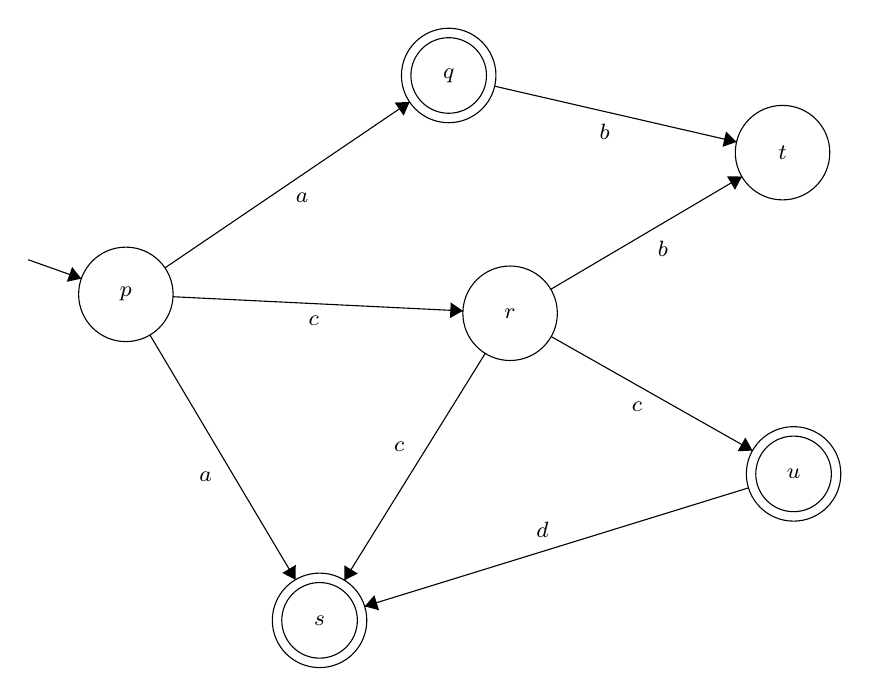
\begin{tikzpicture}[scale=0.2]
				\tikzstyle{every node}+=[inner sep=0pt]
				\draw [black] (9.4,-29.6) circle (3);
				\draw (9.4,-29.6) node {$p$};
				\draw [black] (29.9,-15.7) circle (3);
				\draw (29.9,-15.7) node {$q$};
				\draw [black] (29.9,-15.7) circle (2.4);
				\draw [black] (33.8,-30.8) circle (3);
				\draw (33.8,-30.8) node {$r$};
				\draw [black] (21.7,-50.3) circle (3);
				\draw (21.7,-50.3) node {$s$};
				\draw [black] (21.7,-50.3) circle (2.4);
				\draw [black] (51.1,-20.6) circle (3);
				\draw (51.1,-20.6) node {$t$};
				\draw [black] (51.8,-41) circle (3);
				\draw (51.8,-41) node {$u$};
				\draw [black] (51.8,-41) circle (2.4);
				\draw [black] (3.2,-27.4) -- (6.57,-28.6);
				\fill [black] (6.57,-28.6) -- (5.99,-27.86) -- (5.65,-28.8);
				\draw [black] (11.88,-27.92) -- (27.42,-17.38);
				\fill [black] (27.42,-17.38) -- (26.47,-17.42) -- (27.04,-18.25);
				\draw (20.6,-23.15) node [below] {$a$};
				\draw [black] (10.93,-32.18) -- (20.17,-47.72);
				\fill [black] (20.17,-47.72) -- (20.19,-46.78) -- (19.33,-47.29);
				\draw (14.9,-41.21) node [left] {$a$};
				\draw [black] (12.4,-29.75) -- (30.8,-30.65);
				\fill [black] (30.8,-30.65) -- (30.03,-30.11) -- (29.98,-31.11);
				\draw (21.33,-30.95) node [below] {$c$};
				\draw [black] (32.82,-16.38) -- (48.18,-19.92);
				\fill [black] (48.18,-19.92) -- (47.51,-19.26) -- (47.29,-20.23);
				\draw (39.8,-18.73) node [below] {$b$};
				\draw [black] (36.38,-29.28) -- (48.52,-22.12);
				\fill [black] (48.52,-22.12) -- (47.57,-22.1) -- (48.08,-22.96);
				\draw (43.5,-26.2) node [below] {$b$};
				\draw [black] (36.41,-32.28) -- (49.19,-39.52);
				\fill [black] (49.19,-39.52) -- (48.74,-38.69) -- (48.25,-39.56);
				\draw (41.85,-36.4) node [below] {$c$};
				\draw [black] (48.93,-41.89) -- (24.57,-49.41);
				\fill [black] (24.57,-49.41) -- (25.48,-49.66) -- (25.18,-48.7);
				\draw (35.85,-45.1) node [above] {$d$};
				\draw [black] (32.22,-33.35) -- (23.28,-47.75);
				\fill [black] (23.28,-47.75) -- (24.13,-47.33) -- (23.28,-46.81);
				\draw (27.12,-39.26) node [left] {$c$};
				\end{tikzpicture}
			\end{center}
			\caption{An example of an NFA}
      \label{pic_ex_nfa}
			\end{figure}
%%%end of nfa picture

	\subsection{Deterministic Finite Automaton}
	\label{defDFA}
  A~\emph{deterministic finite automaton} (DFA) is a special case of an NFA, where $\delta$ is a partial function 
$\delta: Q\times \Sigma \to Q$ and $|I| \leq 1$. To be precise, we give the whole definition of DFA.\newline
\newline
		A DFA is a quintuple $\mathcal{A}=(Q,\Sigma,\delta,I,F)$ where
		\begin{itemize}
			\item $Q$ is a finite set of states,
			\item $\Sigma$ is  an alphabet,
			\item $\delta$:  $Q \times \Sigma \to Q$ is a partial transition function, we use $p \xrightarrow{a} q$ to denote that $\delta(p,a)=q$,
			\item $I\subseteq Q$ is finite set of initial states, such that $|I| \leq 1$,
			\item $F\subseteq Q$ is finite set of final states.
		\end{itemize}
    An example of a DFA over $\Sigma=\{a,b,c\}$ is given in Figure \ref{pic_ex_dfa}.


%%%example of DFA
\begin{figure}[t]
\begin{center}
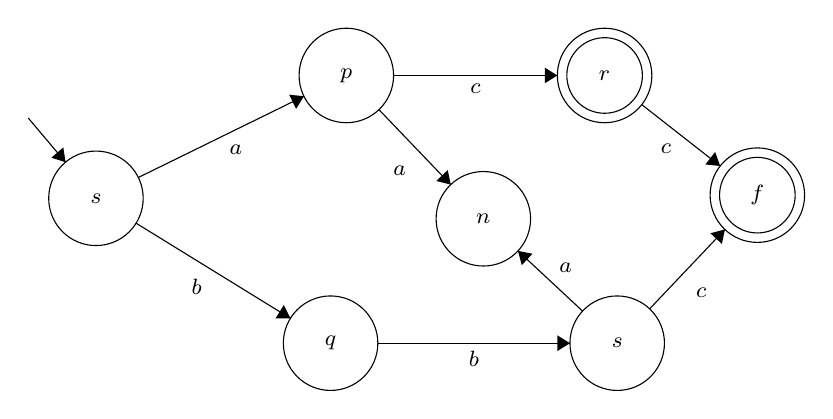
\begin{tikzpicture}[scale=0.2]
\tikzstyle{every node}+=[inner sep=0pt]
\draw [black] (9.9,-28) circle (3);
\draw (9.9,-28) node {$s$};
\draw [black] (25.8,-20.2) circle (3);
\draw (25.8,-20.2) node {$p$};
\draw [black] (24.8,-37.2) circle (3);
\draw (24.8,-37.2) node {$q$};
\draw [black] (42.2,-20.2) circle (3);
\draw (42.2,-20.2) node {$r$};
\draw [black] (42.2,-20.2) circle (2.4);
\draw [black] (43,-37.2) circle (3);
\draw (43,-37.2) node {$s$};
\draw [black] (51.9,-27.8) circle (3);
\draw (51.9,-27.8) node {$f$};
\draw [black] (51.9,-27.8) circle (2.4);
\draw [black] (34.5,-29.3) circle (3);
\draw (34.5,-29.3) node {$n$};
\draw [black] (5.6,-22.9) -- (7.97,-25.71);
\fill [black] (7.97,-25.71) -- (7.83,-24.77) -- (7.07,-25.42);
\draw [black] (12.59,-26.68) -- (23.11,-21.52);
\fill [black] (23.11,-21.52) -- (22.17,-21.42) -- (22.61,-22.32);
\draw (18.79,-24.6) node [below] {$a$};
\draw [black] (12.45,-29.58) -- (22.25,-35.62);
\fill [black] (22.25,-35.62) -- (21.83,-34.78) -- (21.3,-35.63);
\draw (16.3,-33.1) node [below] {$b$};
\draw [black] (28.8,-20.2) -- (39.2,-20.2);
\fill [black] (39.2,-20.2) -- (38.4,-19.7) -- (38.4,-20.7);
\draw (34,-20.7) node [below] {$c$};
\draw [black] (27.8,-37.2) -- (40,-37.2);
\fill [black] (40,-37.2) -- (39.2,-36.7) -- (39.2,-37.7);
\draw (33.9,-37.7) node [below] {$b$};
\draw [black] (45.06,-35.02) -- (49.84,-29.98);
\fill [black] (49.84,-29.98) -- (48.92,-30.22) -- (49.65,-30.9);
\draw (47.98,-33.97) node [right] {$c$};
\draw [black] (44.56,-22.05) -- (49.54,-25.95);
\fill [black] (49.54,-25.95) -- (49.22,-25.06) -- (48.6,-25.85);
\draw (46.09,-24.5) node [below] {$c$};
\draw [black] (27.87,-22.37) -- (32.43,-27.13);
\fill [black] (32.43,-27.13) -- (32.24,-26.21) -- (31.51,-26.9);
\draw (29.62,-26.22) node [left] {$a$};
\draw [black] (40.8,-35.16) -- (36.7,-31.34);
\fill [black] (36.7,-31.34) -- (36.94,-32.25) -- (37.62,-31.52);
\draw (39.72,-32.76) node [above] {$a$};
\end{tikzpicture}
\end{center}
\caption{An example of an DFA}
\label{pic_ex_dfa}
\end{figure}
%%%%end of DFA example

	\subsection{Run of a Finite Automaton}
	\label{defRun}
  A~\emph{run} of an NFA $\mathcal{A}=(Q,\Sigma,\delta,I,F)$ from a state $q$
  over a word $w=a_1\cdots a_n$ is a sequence $r = q_0 \cdots q_n$, where $\forall\,0\leq i \leq n\ .\ q_i\in Q$ 
  such that $q_0=q$ and $q_i\xrightarrow{a_{i+1}}q_{i+1})\in \delta$. 
  The run $r$ is called \emph{accepting} iff $q_n \in F$. 
	A word $w \in \Sigma^{*}$ is called \emph{accepting} if there exists an \emph{accepting} run from some initial state over $w$.
  An \emph{unreachable} state $q$ of an NFA $\mathcal{A}=(Q,\Sigma,\delta,I,F)$ is a state for which there is no run $r=q_0\cdots q$ of 
  $\mathcal{A}$ over a word $w \in \Sigma^{*}$ such that $q_0\in I$.
  An \emph{useless} (also called nonterminating) state $q$ of an NFA $\emph{A}=(Q,\Sigma,\delta,I,F)$ is a state that there is no accepting run $r=q\cdots q_n$ 
  of $\emph{A}$ over a word $w \in \Sigma^{*}$.
  Given a pair of states $p,q\in Q$ of an NFA $\mathcal{A}=(Q,\Sigma,\delta,I,F)$, these states are language equivalent if 
  $\forall w \in \Sigma^{*}: \emph{A run from } p \emph{ over } w \emph{ is accepting} \Leftrightarrow 
			\emph{A run from } q \emph{ over } w \emph{ is accepting}$.


  \subsection{Language of a Finite Automaton}
  Consider a NFA $\mathcal{A}=(Q,\Sigma,\delta,I,F)$.
  The~\emph{language} of a state $q \in Q$ is defined as 
  $L_\mathcal{A}(q) = \{w\in \Sigma^{*}\ |\ $\emph{there exists an accepting run of }$
  \mathcal{A}$$ 
  \emph{ from }q\emph{ over }w\}$, while the language of a set of states $R\subseteq Q$ is defined as $L_{\mathcal{A}}(R)=\bigcup_{q\in R}L_{\mathcal{A}}(q)$.
  The language of an NFA $\mathcal{A}$ is defined as $L_{\mathcal{A}}=L_{\mathcal{A}}(I)$.
  The language of NFA from Figure \ref{pic_ex_nfa} is $L=\{a,cc,ccd\}$.

  \subsection{Complete DFA}
  \label{defCompleteDFA}
  \emph{Complete} DFA $\mathcal{A_C}=(Q_C,\Sigma,\delta_C,I_C,F_C)$ is the DFA where 
  for any $p\in Q_C$, $a\in \Sigma$ exists $q\in Q_C$ such that  $p\xrightarrow{a}q\in\delta_C$. 
  It is possible to transform a DFA $\mathcal{A}=(Q,\Sigma,\delta,I,F)$ to the complete DFA $\mathcal{A_C}=(Q_C,\Sigma,\delta_C,I,F)$ such that $Q_C=Q\cup\{q\}$, 
  $\delta_C = \delta \cup \{p\xrightarrow{a}q\,|\,\nexists\, r \in Q\,.\,p\xrightarrow{a}r\not\in\delta_C\}$.

  \begin{comment}
	\subsection{Minimal DFA}
	\label{defMinDFA}
		A minimal DFA $\mathcal{A}=(Q,\Sigma,\delta,I,F)$ is complete DFA which satisfies these conditions:
		\begin{itemize}
			\item There are no unreachable states,
			\item there is at most one nonterminating state,
			\item there are no two language equivalent states.
		\end{itemize}
  \end{comment}

  \subsection{Operations over Finite Automata}
    \label{defAOps}
    \subsubsection{Automata Union}
    \label{defAUnion}
      Given a pair of NFA $\mathcal{A}=(Q_\mathcal{A},\Sigma,\delta_\mathcal{A},I_\mathcal{A},F_\mathcal{A})$ 
      and $\mathcal{B}=(Q_\mathcal{B},\Sigma,\delta_\mathcal{B},I_\mathcal{B},F_\mathcal{B})$. Their union is defined by
      \begin{description}
        \item $\mathcal{A} \cup \mathcal{B}=(Q_\mathcal{A}\cup Q_\mathcal{B},\Sigma,
            \delta_\mathcal{A}\cup\delta_\mathcal{B},I_\mathcal{A}\cup I_\mathcal{B},F_\mathcal{A}\cup F_\mathcal{B})$
      \end{description}
      Note that $L_{\mathcal{A}\cup\mathcal{B}}=L_\mathcal{A}\cup L_\mathcal{B}$
    
    \subsubsection{Automata Intersection}
    \label{defAInter}
      Given a pair of NFA, $\mathcal{A}=(Q_\mathcal{A},\Sigma,\delta_\mathcal{A},I_\mathcal{A},F_\mathcal{A})$ 
      and $\mathcal{B}=(Q_\mathcal{B},\Sigma,\delta_\mathcal{B},I_\mathcal{B},F_\mathcal{B})$. Their intersection is defined by
      \begin{description}
        \item $\mathcal{A} \times \mathcal{B}=(Q_\mathcal{A}\times Q_\mathcal{B},\Sigma,\delta,I_\mathcal{A}\times I_\mathcal{B},F_\mathcal{A}
          \times F_\mathcal{B})$\
      \end{description}
      where $\delta$ is defined by
      \begin{description}
        \item $\delta = 
        \{(p_1,q_1) \xrightarrow{a} (p_2,q_2)\ |\ p_1 \xrightarrow{a} p_2 \in \delta_\mathcal{A} \wedge q_1 \xrightarrow{a} q_2 \in \delta_\mathcal{B})\}$\
      \end{description}
      Note that $L_{\mathcal{A}\cap\mathcal{B}}=L_\mathcal{A}\cap L_\mathcal{B}$

  \subsubsection{Subset construction}
	\label{subset}
	Now we will define how to construct an equivalent DFA $\mathcal{A}_{det}$ for a given NFA $\mathcal{A}=(Q,\Sigma,\delta,I,F)$. 
  \newline
  \newline
	\label{defSubset}
	$\mathcal{A}_{det}=(2^Q,\Sigma,\delta_{det},I,F_{det})$, where
	\begin{itemize}
		\item $2^Q$ is power set of $Q$, elements of $2^Q$ are called macrostates,
		\item $F_{det}=\{Q'\subseteq Q\ |\ Q'\cap F \not = \emptyset\}$
		\item $\delta_{det}(Q',a)=\bigcup\limits_{q\in Q'}\{r\in Q\,|\,q\xrightarrow{a}r \in \delta\}$.
	\end{itemize}

  This classical (so-called \emph{textbook}) approach is called the \emph{subset construction}.
    An example of this approach is shown in Figure \ref{pic_sub}.
	
	%%%%example of NFA to DFA	
	\begin{figure}[t]
\begin{center}
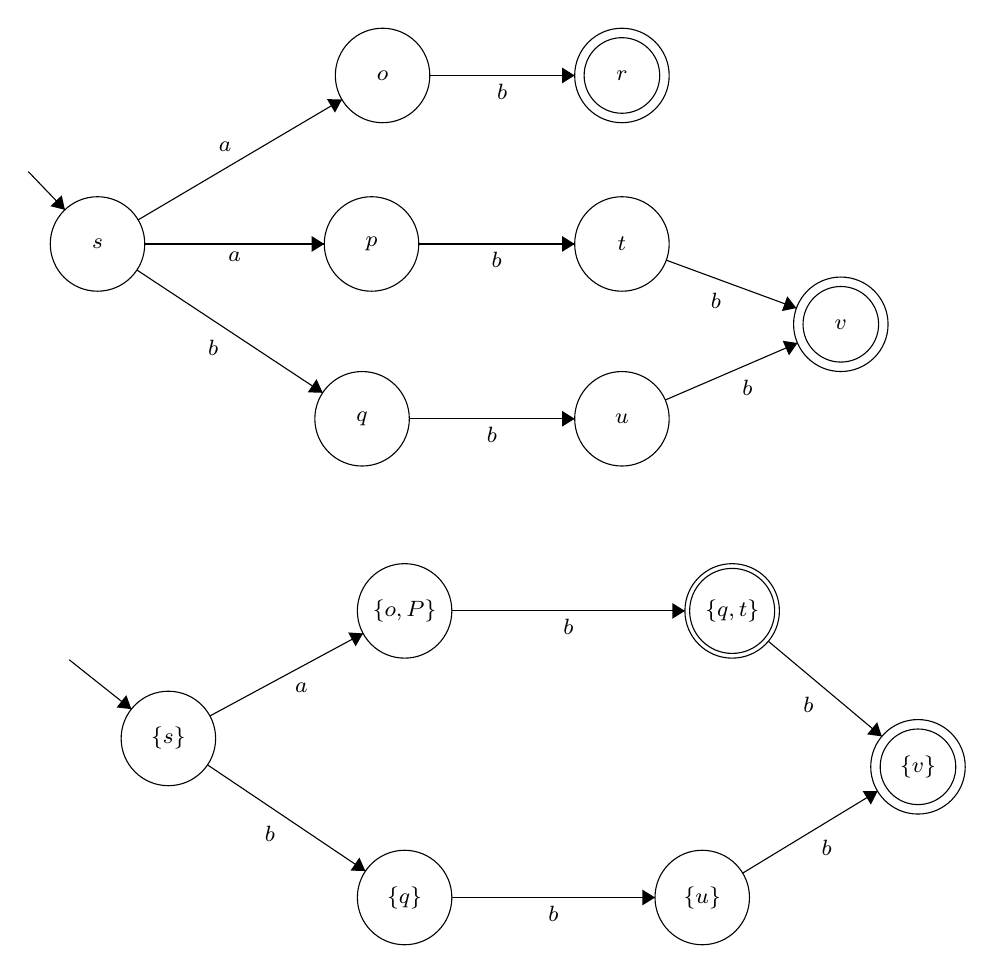
\begin{tikzpicture}[scale=0.2]
\tikzstyle{every node}+=[inner sep=0pt]
\draw [black] (7.9,-14.8) circle (3);
\draw (7.9,-14.8) node {$s$};
\draw [black] (26,-4.1) circle (3);
\draw (26,-4.1) node {$o$};
\draw [black] (25.3,-14.8) circle (3);
\draw (25.3,-14.8) node {$p$};
\draw [black] (24.7,-25.9) circle (3);
\draw (24.7,-25.9) node {$q$};
\draw [black] (41.2,-4.1) circle (3);
\draw (41.2,-4.1) node {$r$};
\draw [black] (41.2,-4.1) circle (2.4);
\draw [black] (41.2,-14.8) circle (3);
\draw (41.2,-14.8) node {$t$};
\draw [black] (41.2,-25.9) circle (3);
\draw (41.2,-25.9) node {$u$};
\draw [black] (55.1,-19.9) circle (3);
\draw (55.1,-19.9) node {$v$};
\draw [black] (55.1,-19.9) circle (2.4);
\draw [black] (12.4,-46.2) circle (3);
\draw (12.4,-46.2) node {$\{s\}$};
\draw [black] (27.4,-38.1) circle (3);
\draw (27.4,-38.1) node {$\{o,P\}$};
\draw [black] (27.4,-56.3) circle (3);
\draw (27.4,-56.3) node {$\{q\}$};
\draw [black] (48.2,-38.1) circle (3);
\draw (48.2,-38.1) node {$\{q,t\}$};
\draw [black] (48.2,-38.1) circle (2.7);
\draw [black] (46.3,-56.3) circle (3);
\draw (46.3,-56.3) node {$\{u\}$};
\draw [black] (60,-48) circle (3);
\draw (60,-48) node {$\{v\}$};
\draw [black] (60,-48) circle (2.4);
\draw [black] (3.5,-10.2) -- (5.83,-12.63);
\fill [black] (5.83,-12.63) -- (5.63,-11.71) -- (4.91,-12.4);
\draw [black] (10.48,-13.27) -- (23.42,-5.63);
\fill [black] (23.42,-5.63) -- (22.47,-5.6) -- (22.98,-6.46);
\draw (16,-8.95) node [above] {$a$};
\draw [black] (10.9,-14.8) -- (22.3,-14.8);
\fill [black] (22.3,-14.8) -- (21.5,-14.3) -- (21.5,-15.3);
\draw (16.6,-15.3) node [below] {$a$};
\draw [black] (10.4,-16.45) -- (22.2,-24.25);
\fill [black] (22.2,-24.25) -- (21.81,-23.39) -- (21.25,-24.22);
\draw (15.25,-20.85) node [below] {$b$};
\draw [black] (29,-4.1) -- (38.2,-4.1);
\fill [black] (38.2,-4.1) -- (37.4,-3.6) -- (37.4,-4.6);
\draw (33.6,-4.6) node [below] {$b$};
\draw [black] (28.3,-14.8) -- (38.2,-14.8);
\fill [black] (38.2,-14.8) -- (37.4,-14.3) -- (37.4,-15.3);
\draw (33.25,-15.3) node [below] {$b$};
\draw [black] (27.7,-25.9) -- (38.2,-25.9);
\fill [black] (38.2,-25.9) -- (37.4,-25.4) -- (37.4,-26.4);
\draw (32.95,-26.4) node [below] {$b$};
\draw [black] (43.95,-24.71) -- (52.35,-21.09);
\fill [black] (52.35,-21.09) -- (51.41,-20.95) -- (51.81,-21.87);
\draw (49.17,-23.41) node [below] {$b$};
\draw [black] (44.02,-15.83) -- (52.28,-18.87);
\fill [black] (52.28,-18.87) -- (51.7,-18.12) -- (51.36,-19.06);
\draw (47.17,-17.88) node [below] {$b$};
\draw [black] (6.1,-41.2) -- (10.05,-44.34);
\fill [black] (10.05,-44.34) -- (9.73,-43.45) -- (9.11,-44.23);
\draw [black] (15.04,-44.77) -- (24.76,-39.53);
\fill [black] (24.76,-39.53) -- (23.82,-39.47) -- (24.29,-40.35);
\draw (20.85,-42.65) node [below] {$a$};
\draw [black] (14.89,-47.88) -- (24.91,-54.62);
\fill [black] (24.91,-54.62) -- (24.53,-53.76) -- (23.97,-54.59);
\draw (18.85,-51.75) node [below] {$b$};
\draw [black] (30.4,-38.1) -- (45.2,-38.1);
\fill [black] (45.2,-38.1) -- (44.4,-37.6) -- (44.4,-38.6);
\draw (37.8,-38.6) node [below] {$b$};
\draw [black] (30.4,-56.3) -- (43.3,-56.3);
\fill [black] (43.3,-56.3) -- (42.5,-55.8) -- (42.5,-56.8);
\draw (36.85,-56.8) node [below] {$b$};
\draw [black] (48.87,-54.75) -- (57.43,-49.55);
\fill [black] (57.43,-49.55) -- (56.49,-49.54) -- (57.01,-50.4);
\draw (54.2,-52.65) node [below] {$b$};
\draw [black] (50.5,-40.03) -- (57.7,-46.07);
\fill [black] (57.7,-46.07) -- (57.41,-45.17) -- (56.77,-45.94);
\draw (53.04,-43.54) node [below] {$b$};
\end{tikzpicture}
\end{center}
	\caption{A simple example of NFA to DFA conversion via the subset construction with the reduction of inaccessible state. 
   A small NFA with a small $\Sigma$ is shown here, but for larger NFA could state explosion occur.}
    \label{pic_sub}
	\end{figure}
	%%%end of NFA to DFA

  \section{Regular Languages}
		A language $L$ is \emph{regular} if there exists an NFA $\mathcal{A}=(Q,\Sigma,\delta,I,F)$, such that $L=L_\mathcal{A}$.

    \subsection{Closure Properties}
    The class of regular languages is closed under certain operation if the result of this operation on some regular language is always a regular language too.

		Let us introduce the closure properties of regular languages on an alphabet $\Sigma$:
		\begin{itemize}
			\item Union:  $L=L_1 \cup L_2$. Union of two NFA is described in section \ref{defAUnion}.
			\item Intersection:  $L=L_1 \cap L_2$. Intersection of two NFA is described in section \ref{defAInter}.
			\item Complement: $L=\overline{L_1}$.
      Complement of NFA $\mathcal{A}$ is done by its determinizing (via subset construction described in section \ref{subset}), completion of this DFA (via
      method described in \ref{defCompleteDFA}) and swapping its final and non-final states set.

      \item Difference: $L=L_1-L_2$. Difference of NFA $\mathcal{A}=(Q_\mathcal{A},\Sigma,\delta_\mathcal{A},I_\mathcal{A},F_\mathcal{A})$ 
      and NFA $\mathcal{B}=(Q_\mathcal{B},\Sigma,\delta_\mathcal{B},I_\mathcal{B},F_\mathcal{B})$ is done by creating
      complete DFA $\mathcal{B_C}$ (by methods \ref{subset} and \ref{defCompleteDFA}) then complementing $\mathcal{B_C}$ and
      finally creating intersection $\mathcal{A}\cap\overline{\mathcal{B_C}}$.

			\item Reversal: $L=\{a_1\dots a_n \in \Sigma^{*} \ |\ y=a_n\dots a_1 \in L\}$.
      Reversion of a NFA $\mathcal{A}=(Q_\mathcal{A},\Sigma,\delta_\mathcal{A},I_\mathcal{A},F_\mathcal{A})$ is
      NFA $\mathcal{A}_{rev}=(Q_{\mathcal{A}},\Sigma,\delta_{\mathcal{A}_{rev}},F_{\mathcal{A}},I_{\mathcal{A}})$ 
      where $\delta_{\mathcal{A}_{rev}}=\{(q,a,p)\,|\,p,q \in Q_\mathcal{A}, a \in \Sigma\,.\,p\xrightarrow{a}q\in\delta_{\mathcal{A}}\}$ .

      \item Iteration: $L^{*}$.
      Iteration of a NFA $\mathcal{A}=(Q_\mathcal{A},\Sigma,\delta_\mathcal{A},I_\mathcal{A},F_\mathcal{A})$ 
      is NFA $\mathcal{A}^{*}=(Q_\mathcal{A},\Sigma,\delta_\mathcal{A}^{*},I_\mathcal{A},F_\mathcal{A}\cup I_\mathcal{A})$ 
      where $\delta_\mathcal{A}^{*}=\delta_\mathcal{A}\cup
      \{q\xrightarrow{a}i\,|\,f\in F_\mathcal{A},i\in I_\mathcal{A}\,.\,q\xrightarrow{a}f \in \delta_\mathcal{A}\}$

			\item Concatenation: $L\cdot K=\{x \cdot y\ |\ x\in L \wedge y\in K\}$.
      Concatenation of a NFA $\mathcal{A}=(Q_\mathcal{A},\Sigma,\delta_\mathcal{A},I_\mathcal{A},F_\mathcal{A})$ and a NFA 
      $\mathcal{B}=(Q_\mathcal{B},\Sigma,\delta_\mathcal{B},I_\mathcal{B},F_\mathcal{B})$ is 
      NFA $\mathcal{A}\cdot\mathcal{B}=(Q_\mathcal{A}\cup Q_\mathcal{B},\Sigma,\delta,I_\mathcal{A},F_\mathcal{B})$ where $\delta=\delta_\mathcal{A} \cup
      \{q\xrightarrow{a}i\,|\,f\in F_\mathcal{A},i\in I_\mathcal{B}\,.\,q\xrightarrow{a}f \in \delta_\mathcal{A}\}$

  \end{itemize}

\begin{comment}
		\subsection{Union, intersection, inclusion}
\label{defOP}
		\begin{definition}
		Let $L_1$ and $L_2$ be languages. \emph{Union, intersection, inclusion} are defined as:
		\begin{description*}
			\item [$Union:$]  $L_1 \cup L_2=\{x\ |\ x \in L_1 \vee x\in L_2\}$
			\item [$Intersection:$]  $L_1 \cap L_2=\{x\ |\ x \in L_1 \wedge x\in L_2\}$
			\item [$Inclusion:$]  $L_1 \subseteq L_2 \Leftrightarrow L_1 \cap \overline{L_2}=\varnothing$
		\end{description*}
		\end{definition}
		
\end{comment}

\chapter{Checking Inclusion over NFA}
\label{chapInclusion}
Given a pair of NFA $\mathcal{A}=(Q_\mathcal{A},\Sigma,\delta_\mathcal{A},I_\mathcal{A},F_\mathcal{A})$ 
and $\mathcal{B}=(Q_\mathcal{B},\Sigma,\delta_\mathcal{B},I_\mathcal{B},F_\mathcal{B})$, 
the \emph{language inclusion problem} is deciding whether $L_\mathcal{A} \subseteq L_\mathcal{B}$.
This problem is PSPACE-complete \cite{cav06}. The \emph{textbook} algorithm for checking inclusion $L_\mathcal{A}\subseteq L_\mathcal{B}$ 
is based on the observation that this holds iff $L_{\mathcal{A}}\cap L_\mathcal{B}=\emptyset$ and works by first 
determinizing $\mathcal{B}$ (yielding the DFA 
$\mathcal{B}_{det}$ using the subset construction algorithm presented in section \ref{subset}), 
complementing it (yielding $\overline{\mathcal{B}_{det}}$) and constructing the NFA $\mathcal{A} \cap \overline{\mathcal{B}_{det}}$ 
accepting the intersection of $L_{\mathcal{A}}$ and ${L_{\overline{\mathcal{B}_{det}}}}$ and
checking whether its language is nonempty. Any accepting run in this automaton may serve as a witness that the inclusion between $\mathcal{A}$ 
and $\mathcal{B}$ does not hold.
Some recently introduced approaches (the so-called antichains \cite{cav06}, its optimization using simulation \cite{tacas10}, and the so-called bisimulation up to
congruence \cite{popl13}) avoid the explicit construction of $\overline{\mathcal{B}_{det}}$ and the related state explosion in many cases.

We have to define the following terms for the further description of the new techniques for the inclusion checking.
We denote a product state of a NFA $\mathcal{A} \cap \mathcal{B}_{det}$ as a pair $(p,P)$ of a state $p\in Q_\mathcal{A}$ and a 
macrostate $P \subseteq Q_{\mathcal{B}_{det}}$.
We define the post-image of a product state $(p,P)$ of a NFA $\mathcal{A}\cap \mathcal{B}$ by
$Post(p,P):=\{(p',P')\ |\ \exists\, a \in \Sigma: p\xrightarrow{a} p' \in \delta_\mathcal{A}, P'=
\{p''\in Q_\mathcal{B}\ |\ \exists p''' \in P:p'''\xrightarrow{a} p''\in \delta_\mathcal{B}\}\}$

\section{Checking Inclusion with Antichains and Simulation}
\label{sectionAntichain}
We define an antichain, simulation and some others terms before describing the algorithm itself.
Given a partially ordered set $Y$, an \emph {antichain} is a set $X \subseteq Y$ such that all elements of $X$ are incomparable.
A~forward \emph{simulation} on an NFA $\mathcal{A}=(Q_\mathcal{A},\Sigma,\delta_\mathcal{A},I_\mathcal{A},F_\mathcal{A})$ 
is a relation $\preceq\  \subseteq Q_\mathcal{A} \times Q_\mathcal{A}$ 
such that if $p \preceq r$ then (i) $p \in F_\mathcal{A} 
\Rightarrow r \in F_\mathcal{A}$ and (ii) for every transition $p\xrightarrow{a}p' \in \delta_\mathcal{A}$, there exists a transition 
$r\xrightarrow{a}r' \in \delta_\mathcal{A}$ such that $p' \preceq r'$  \cite{focs95}. 
Note that simulation implies language inclusion, i.e., $p\preceq q \Rightarrow L_\mathcal{A}(p)
\subseteq L_\mathcal{A}(q)$. 
%Let denote $A^{\subseteq}$ as the set of relations over automaton $A$ that imply inclusion,\\ so if $\preceq \in A^{\subseteq}$, 
%then $p\preceq r \Rightarrow L(A)(p) \subseteq L(A)(r)$.
%
For two macro-states $P$ and $R$ of a NFA is $R\preceq^{\forall\exists}P$ shorthand for $\forall r\in R.\exists p \in P: r \preceq p$.
Macrostate $P$ of a NFA is final if there exists $p\in P$ which is final state of this NFA.
%A product state $(p,P)$ of a NFA $\mathcal{A} \cap \mathcal{B}_{det}$ is final, if $p$ is final in automaton $\mathcal{A}$ 
%and $P$ is not final in automaton $\mathcal{B}$. %TODO zamyslet se nad definici final makrostavu

\subsection{Antichains Algorithm Description}
The Antichains algorithm \cite{cav06} described in pseudocode in Algorithm \ref{algAntichain} 
starts searching for a final state of the product automaton $\mathcal{A}\cap \overline{\mathcal{B}_{det}}$ while
pruning out the states which are not necessary to explore. $\mathcal{A}$ is explored nondeterministically and $\mathcal{B}$ 
is gradually determinized, so the algorithm explores pairs $(p,P)$ where $p\in Q_\mathcal{A}$ and $P \subseteq Q_\mathcal{B}$. 
The antichains algorithm derives new states along the product automaton transitions and inserts them to the set of pairs $Next$ for further processing. 
Once a product state from $Next$ is processed and its post-image is created the product state is moved to the set of visited pairs $Processed$.
$Next$ and $Processed$ keeps only minimal elements with respect to the ordering given by $(r,R)\sqsubseteq (p,P)$ iff $r=p \wedge R \subseteq P$. 
If there is a pair $(p,P)$ generated and there is 
$(r,R)\in Next\cup Processed$ such that $(r,R) \sqsubseteq (p,P)$, we can skip $(p,P)$ and not insert it to $Next$ for further search.
 
An improvement of the antichains algorithm using simulation \cite{tacas10} is based on the following optimization. 
We can stop the search from a pair $(p,P)$ if either (a) there exists some already visited pair $(r,R) \in Next\cup Processed$ 
such that $p\preceq r \wedge R\preceq^{\forall\exists}P$, 
or (b) there is $p' \in P$ such that $p \preceq p'$. This first
optimization is at lines 11--14 in the pseudocode.

Another optimization \cite{tacas10} of the antichain algorithm is based on the fact 
that $L_\mathcal{A}(P)=L_\mathcal{A}(P-\{p_1\})$ if there exists $p_2 \in P-\{p_1\}$, such that $p_1 \preceq p_2$. We can remove the state $p_1$ 
from macrostate $P$, because if $L_\mathcal{A}(P)$ does not contain the word 
then $L_\mathcal{A}(P-\{p_1\})$ does not contains it either. This optimization is applied by the function $Minimize$ at
the lines 4 and 7 in the pseudocode.

\begin{figure}[bt]
\begin{algorithm}[H]
	\label{algAntichain}
	\KwIn{NFAs $\mathcal{A}=(Q_\mathcal{A},\Sigma,\delta_\mathcal{A},I_\mathcal{A},F_\mathcal{A}),\ 
    \mathcal{B}=(Q_\mathcal{B},\Sigma,\delta_\mathcal{B},I_\mathcal{B},F_\mathcal{B})$.\\ 
	 A relation $\preceq$ over $\mathcal{A} \cup \mathcal{B}$ that imply language inclusion.}
	\KwOut{TRUE if $\mathcal{L_\mathcal{A}}\subseteq\mathcal{L_\mathcal{B}}$. Otherwise FALSE.}
		\If{there is a final product-state in \{$(i,I_{\mathcal{B}})\,|\,i\in I_{\mathcal{A}}$\}}
			{return FALSE\;}
		$Processed$:=$\varnothing$\;
    %$Next$:= Initialize(\{$(s,Minimize(I_B))\mid s\in I_A$\})\;
		$Next$:= \{$(s,Minimize(I_B))\mid s\in I_A$\}\;
		\While{$Next\neq \emptyset$}
		{
			Pick and remove a product-state $(r,R)$ from $Next$ and move it to $Processed$\;
			\ForEach{$(p,P)\in \{(r',Minimize(R'))\mid (r',R')\in Post((r,R))\}$}
			{
				\eIf{$(p,P)$ is a final product-state}
				{
					\Return FALSE\;}
					{
						\If{$\not{\exists}p'\in P\ s.t.\ p\preceq p'$}
						{
							\If{$\not{\exists} (x,X) \in Processed\cup Next\ s.t.\ p\preceq x \wedge X\preceq^{\forall \exists}P$}
							{
							 Remove all $(x,X)$ from $Processed\cup Next\ s.t.\ x\preceq p \wedge P\preceq^{\forall \exists}X$\;
							 Add $(p,P)$ to $Next$\;
							}
						}
				 }
		  }
		}
		\Return TRUE;
	\caption{Language inclusion checking with antichains and simulations}
\end{algorithm}
\end{figure}

\begin{comment}
Let describe two optimization use in algorithm \ref{algAntichain} based on \cite{tacas10}. First optimization comes from the observation that
we can stop search from product-state $(p,P)$, if there exists some visited product state $(r,R)$, 
such that $p\preceq r \wedge R\preceq^{\forall\exists}P$, or $\exists p'\in P: p \preceq p'$. First part of condition says that 
if $(p,P)$ takes automaton to the accepting state, $(r,R)$ will be taken to accepting state too, so we do not have search from $(p,P)$. Second part of condition
shows, that every accepting word of $p$ takes $P$ to accepting state too, because $\exists p'\in P: p \preceq p'$.
Proof for this can be found in \cite{tacas10}. This first
optimization is in algorithm \ref{algAntichain} at lines 11--14.

Second optimization is based on fact, that $L(A)(P)=L(A)(P-\{p_1\})$, if there exists $p_2$, such as $p_1 \preceq p_2$. We can remove the state $p_1$ 
from macro-state $P$, because if $L(A)(P)$ rejects the word, then $L(A)(P-\{p_1\})$ rejects this word too. This optimization is applied in function $Minimize$ at
lines 4 and 7 in algorithm \ref{algAntichain}. Proof for this optimization is again in \cite{tacas10}.
\end{comment}

\section{Checking Inclusion with Bisimulation up to Congruence}
\label{sectionCongr}
Another approach to checking language inclusion of NFA is based on bisimulation up to congruence \cite{popl13}.
Given a set $X$ and an n-ary operation $O$ over $X$, an equivalence relation $\sim_R$ is a congruence if $\forall a_1,\ldots,a_n,b_1,\ldots,b_n\in X$:
		\begin{description}
			\item $a_1 \sim_{R} b_1,\ldots,a_n \sim_{R} b_n \Rightarrow O(a_1,\ldots,a_n) \sim_{R} O(b_1,\ldots,b_n)$
		\end{description}
Given an NFA $\mathcal{A}=(Q_\mathcal{A},\Sigma,\delta_\mathcal{A},I_\mathcal{A},F_\mathcal{A})$ and a relation 
$R\subseteq Q_\mathcal{A}\times Q_\mathcal{A}$. $R$ is bisimulation if both $R$ and $R^{-1}$ are simulations on the the NFA $\mathcal{A}$.

The presented technique was originally developed for checking equivalence of languages of automata but it can
also be used for checking language inclusion, based on the observation that $L_\mathcal{A}\cup L_\mathcal{B}= L_\mathcal{B}$ iff 
$L_\mathcal{A}\subseteq L_\mathcal{B}$.

  This approach is based on the computation of a~\emph{congruence closure} $c(R)$ 
  for some binary relation $R$ on the states of the determinized automaton $R \subseteq 2^Q\times 2^Q$ defined 
  %associative, commutative, idempotent binary operation $+: Q\times Q \to Q$ 
  as a relation $c(R)=(r\cup s\cup t \cup u\cup id)^{\omega}(R)$, where
  \begin{description}
  \item $id(R)=R$, 
  \item $r(R)=\{(X,X)\ |\ X\subseteq Q\}$, 
  \item $s(R)=\{(Y,X)\ |\ XRY\}$,
  \item $t(R)=\{(X,Z)\ |\ \exists\,Y\subseteq Q,\ XRYRZ\}$,
  \item $u(R)=\{(X_1 \cup X_2,Y_1\cup Y_2)\ |\ X_1 R Y_1 \wedge X_2 R Y_2\}$. 
  \end{description}



 \subsection{Congruence Algorithm Description}
\label{subsectCongr}
The congruence algorithm works on a similar principle as the antichains algorithm but  %dodefinovat bisimulaci
it tries to build bisimulation that relates $\mathcal{A}$ and $\mathcal{B}$. The algorithm starts building not only $\mathcal{B}_{det}$ 
but also $\mathcal{A}_{det}$ because the original purpose of this algorithm is checking of 
language equivalence. States of the product automaton $\mathcal{A}_{det} \times \mathcal{B}_{det}$  (so-called product states) are the pairs 
$(P_\mathcal{A},P_\mathcal{B})$ of a macrostate $P_\mathcal{A} \subseteq Q_\mathcal{A}$ and a macrostate
$P_\mathcal{B} \subseteq Q_\mathcal{B}$. 
The algorithm searches for a victim that proves $L_\mathcal{A} \neq L_\mathcal{B}$. The victim is a product state $(P_\mathcal{A},P_\mathcal{B})$ 
which breaks a condition that
the $P_\mathcal{A}$ contains a final state of $A$ if and only if $P_\mathcal{B}$ contains a final state of $B$. 

The optimization brought by this algorithm is based on computing a congruence closure of the set of already visited pairs of macrostates. 
If the generated pair is in the congruence closure, it can be skipped and further not processed.
The whole pseudocode of the congruence algorithm is given in Algorithm \ref{algCongr}. The operation post on a product state $(P,Q)$ of a 
NFA $\mathcal{A}\cap \mathcal{B}$ used in the pseudocode we define by:\
$Post((P,Q)):=\{(P',Q')\ |\ \exists a \in \Sigma: P'=
\{p''\in Q_\mathcal{B}\ |\ \exists p \in P:p\xrightarrow{a} p''\in \delta_\mathcal{B}\}, Q'=
\{q''\in Q_\mathcal{B}\ |\ \exists q \in Q:q\xrightarrow{a} q''\in \delta_\mathcal{B}\}\}$


\begin{figure}[ht]
	\begin{algorithm}[H]
		\label{algCongr}
		\KwIn{NFAs $\mathcal{A}=(Q_\mathcal{A},\Sigma,\delta_\mathcal{A},I_\mathcal{A},F_\mathcal{A}),\
      B=(Q_\mathcal{B},\Sigma,\delta_\mathcal{B},I_\mathcal{B},F_\mathcal{B})$.} 
		\KwOut{TRUE, if $L_\mathcal{A}=L_\mathcal{B}$. Otherwise FALSE.}
			$Processed$ := $\emptyset$\;
			$Next$ := $(I_\mathcal{A},I_\mathcal{B})$\;
			\While{$Next \neq \emptyset$}
			{
				Pick and remove a product state $(X,Y)$ from $Next$\;
				\If {($X$,$Y) \in c(Processed \cup Next)$}
				{continue\;}
				\If {$(X\cap F_\mathcal{A}\ \neq \emptyset) \Leftrightarrow (Y\cap F_\mathcal{B} \neq \varnothing)$}
				{
					\Return FALSE\;
				}
				%\ForAll {$a\in \Sigma$}
				%{
					Add elements from $Post(X,Y)$ to $Next$\;
				%}
				Add $X$,$Y$ to $Processed$\;
			}
			\Return TRUE;
		\caption{Language equivalence checking with congruence}
\end{algorithm}
\end{figure}

\begin{figure}[th]
\begin{center}
	\scalebox{1}
	{
		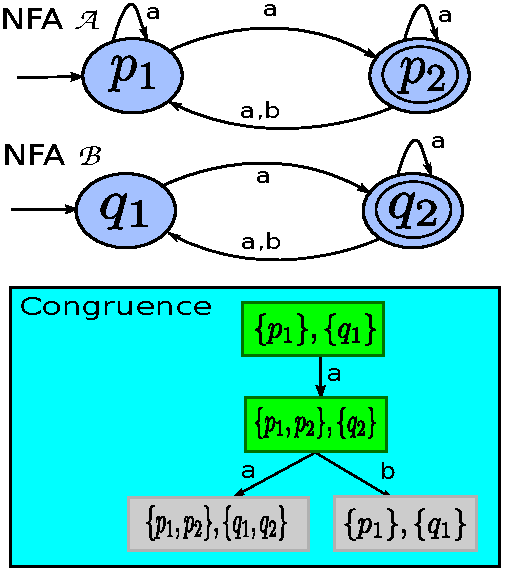
\includegraphics[scale=0.5]{fig/congr1.pdf}
		\hspace{0.55cm}
  	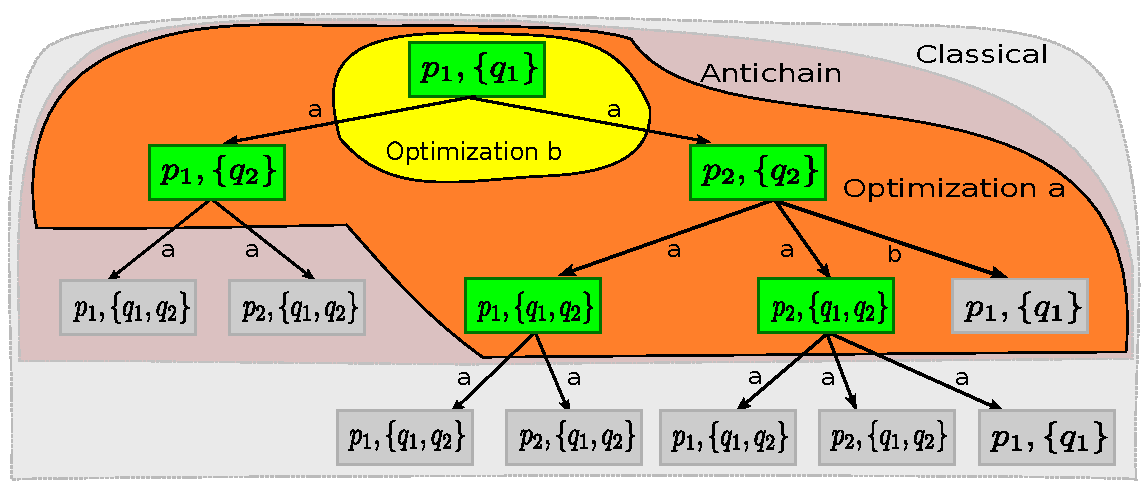
\includegraphics[scale=0.5]{fig/ac1.pdf}
	}
  \caption{
      \rm{
      \hspace{0.1cm} The figure is based on an example from \cite{tacas10}.
      It shows the procedure of checking language inclusion between two NFA using the mentioned approaches (which correspond to the labeled areas).
      %The labeled areas correspond to mentioned approaches.
      The antichains algorithm reduces number of the generated states compared with the classical,
      e.g., $(p_2,\{q_1,q_2\})$ is not further explored because $(p_2,\{q_2\}) \sqsubseteq (p_2,\{q_1,q_2\})$. 
      The optimization a) and b) are improvements of the antichains algorithm using simulation. 
      The congruence algorithm also reduces the number of the generated states, so $(\{p_1,p_2\},\{q_1,q_2\})$ 
      is not further explored because it is in the congruence closure 
      of the set of visited pairs of states.}}
      %It shows macrostates 
			%that are generated when checking language inclusion between two NFA using different approaches. Optimization a and b
			%correspond to the parts of the improvement of antichain algorithm using simulation.}}
  \label{automata}
\end{center}
\end{figure}
Comparison of the mentioned approaches to checking language inclusion can be seen in Figure \ref{automata}.

\subsection{Computation of Congruence Closure}
\label{subsectionCongr}
The computation of the congruence closure is crucial for performance and efficiency of the whole method. The work described in this thesis implements
an algorithm introduced in \cite{popl13} which is based on the use of the so-called rewriting rules. For each pair of macrostates $(X,Y)$ in 
a relation $R$ of the visited macrostates there exist two rewriting rules which have following form:
\begin{center}
$X\rightarrow X\cup Y$ \hspace{5cm} $Y\rightarrow X\cup Y$
\end{center}

These rules can be used for computation of a \emph{normal form} of a set of states \cite{popl13}. The normal form of a set is the
largest set of its equivalence classes \cite{popl13}. The normal form of a macrostate $X$ created with
the rewriting rules of the relation $R$ is denoted as $X{\downarrow_R}$.
Checking if $(X,Y)\in c(R)$ using derivation of the normal form is based on the observation that $X{\downarrow_R}=Y{\downarrow_R}$ 
iff $(X,Y)\in c(R)$ \cite{popl13}.

An example (taken from \cite{popl13}) is given to illustrate an application of this approach for checking equivalency of 
NFA $\mathcal{A}=(Q_\mathcal{A},\Sigma,\delta_\mathcal{A},I_\mathcal{A},F_\mathcal{A})$ 
and $\mathcal{B}=(Q_\mathcal{B},\Sigma,\delta_\mathcal{B},I_\mathcal{B},F_\mathcal{B})$ (both NFA are in Figure \ref{figHKCex}). 
Consider a relation $R=\{(\{x\},\{u\}),(\{y,z\},\{u\})\}$ of the visited product states and a newly generated product state 
$(\{x,y\},\{u\})$ (where $\{x,y\}\subseteq Q_\mathcal{A}$ and 
$\{u\} \subseteq Q_\mathcal{B}$). For checking whether $(\{x,y\},\{u\})\in c(R)$ it is needed to compute the normal forms of the macrostates $\{x,y\}$ and $\{u\}$ 
A derivation of both normal forms is shown in Figure \ref{figHKCRew}. 
The normal form of the set $\{x,y\}$ is derived in two steps.
At the first step the rule $\{x\}\rightarrow\{x,u\}$ is applied (based on the pair $(\{x\},\{u\})\in R$) so we get a set $\{x,y,u\}$. As the second one, the rule 
$\{u\}\rightarrow\{y,z,u\}$ (based on the product state $(\{y,z\},\{u\})\in R$) is applied, so the result is $\{x,y,z,u\}$. The normal form of the set $\{u\}$
is derived in two steps too. At the first step, the rule $\{u\}\rightarrow\{x,u\}$ is applied so we get a set $\{x,u\}$ and then the rule 
$\{u\}\rightarrow\{y,z,u\}$ is used and the result set is $\{x,y,z,u\}$. The derived normal sets are equal so it holds that $(\{x,y\},\{u\})\in c(R)$ and
it is not necessary to further explore the product automaton $\mathcal{A}\times \mathcal{B}$ from this state.

\begin{figure}[tb]
\begin{center}
  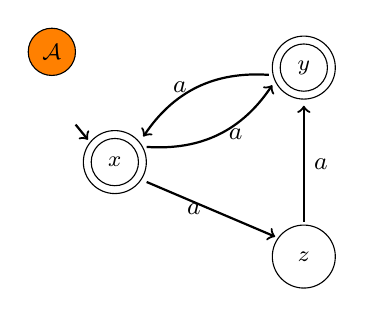
\begin{tikzpicture}
[
  scale=0.4
]

\draw (2,8.5)[fill=orange] circle (0.75);
\draw (2,8.5) node {$\mathcal{A}$};

\draw (4,5) circle (1);
\draw (4,5) circle (0.75);
\draw (4,5) node {$x$};
\draw (10,8) circle (1);
\draw (10,8) circle (0.75);
\draw (10,8) node {$y$};
\draw (10,2) circle (1);
\draw (10,2) node {$z$};

\node (s) at (2.5,6.5) {};
\node (sx) at (3.4,5.4) {};

\node (x) at (4.7,5.5) {};
\node (y) at (9.2,7.75) {};

\node (xz) at (4.7,4.5) {};
\node (z) at (9.4,2.5) {};

\node (yz) at (10,7.1) {};
\node (zy) at (10,2.8) {};

\path[->,thick,every node/.style={font=\sffamily\small}]
(x) edge [bend right] node[right] {$a$} (y)
(y) edge [bend right] node[left] {$a$} (x)

(xz) edge node[left] {$a$} (z)

(zy) edge node[right] {$a$} (yz)

(s) edge (sx);

\end{tikzpicture}

  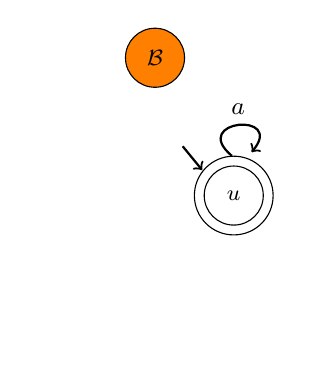
\begin{tikzpicture}
[
  scale=0.5
]

\node (start) at(-1,1) {};
\draw (2,8.5)[fill=orange] circle (0.75);
\draw (2,8.5) node {$\mathcal{B}$};

\draw (4,5) circle (1);
\draw (4,5) circle (0.75);
\draw (4,5) node {$u$};

\node (s) at (2.5,6.5) {};
\node (sx) at (3.4,5.4) {};

\node (x) at (4.2,5.8) {};
\node (x1) at (4.4,4.3) {};

\path[->,thick,every node/.style={font=\sffamily\small}]
  (x) edge [out=140, in=50, loop] node[above] {$a$} (x)

  (s) edge (sx);
\end{tikzpicture}

    \caption{The figure shows two NFA $\mathcal{A}$, $\mathcal{B}$ 
      which are used in the example describing computation of a congruence closure in Figure \ref{figHKCRew}}
		\label{figHKCex}
\end{center}
\end{figure}

\begin{figure}[bt]
  \begin{center}
    \begin{tikzpicture}[scale=0.12]
    \tikzstyle{every node}+=[inner sep=0pt]
    \draw (-20,0) node {\textit{\textcolor{Green}{$\{x,y\}$}}};
    \node (xy) at (-20,-2) {};  
    \draw (34,0) node {\textit{\textcolor{blue}{$\{u\}$}}};
    \node (u) at (32,-2) {};  

    \node (xyuU) at (-12,-8) {}; 
    \draw (-10,-10) node {\textit{\textcolor{Green}{$\{x,y,u\}$}}};
    \node (xyuP) at (-6,-12) {};

    \node (xuU) at (25,-8) {}; 
    \draw (22,-10) node {\textit{\textcolor{blue}{$\{x,u\}$}}};
    \node (xuP) at (20,-12) {}; 

    \node (xyzu) at (5,-18) {};
    \node (xyzu1) at (9,-18) {};
    \node (xyzu2) at (45,-18) {};
    \draw (7,-20) node {\textit{\textcolor{red}{$\{x,y,z,u\}$}}};

    
    \draw[->,thick,dashed] (xy) -- (xyuU);
    \draw[->,thick,dashed] (xyuP) -- (xyzu);
    \draw[->,thick,dashed] (u) -- (xuU);
    \draw[->,thick,dashed] (xuP) -- (xyzu1);
\end{tikzpicture}

    \caption{Derivation of the normal forms of the sets $\{x,y\}$ and $\{u\}$ using rewriting
      rules of the macrostates of a relation $R=\{(\{x\},\{u\}),(\{y,z\},\{u\})\}$.}
    \label{figHKCRew}
  \end{center}
\end{figure}

A problem of this approach is that we do not know which rules of the relation $R$ to use, in which order to use the 
and each rule can be used only once for computing the normal form. 
Due to this conditions the time complexity for finding an applicable rule is in the worst case $|R|\cdot|Q|$ where $Q$ is a set of states of a NFA.
The whole derivation of the normal set is bounded by the complexity $|R|^2 \cdot |Q|$ because we can apply at most $r$ rules \cite{popl13}.

\subsubsection{Optimization for Inclusion Checking}
\label{congrOpt}
\begin{figure}[bt]
  \begin{center}
    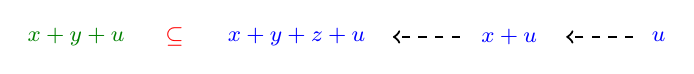
\begin{tikzpicture}[scale=0.1]
  \tikzstyle{every node}+=[inner sep=0pt]
  \draw (-30,0) node {\textit{\textcolor{Green}{$x+y+u$}}};
  \node (xy) at (-10,0) {};  
  \draw (-17.5,0) node {\textcolor{red}{$\subseteq$}};
  \draw (-2,0) node {\textit{\textcolor{blue}{$x+y+z+u$}}};
  \node (xmax) at (10,0) {};  
  \node (x+uP) at (19,0) {};  
  \draw (25,0) node {\textit{\textcolor{blue}{$x+u$}}};
  \node (x+u) at (32,0) {};  
  \draw (44,0) node {\textit{\textcolor{blue}{$u$}}};
  \node (u) at (41,0) {};  
  
  \draw[->,thick,dashed] (u) -- (x+u) ;
  \draw[->,thick,dashed] (x+uP) -- (xmax) ;
\end{tikzpicture}

    \caption{The figure shows the deriving of the normal form the set $\{u\}$ using rewriting
      rules of the elements of a relation $R=\{(\{x,u\},\{u\}),(\{y,z,u\},\{u\})\}$.}
    \label{figHKCRewO}
  \end{center}
\end{figure}
Since the algorithm based on bisimulation up to congruence is primarily used for checking equivalence of NFA, it is possible to make some simplifications for
checking inclusion. An optimization is possible in checking whether a macrostate $(X,Y)$ is in the congruence closure of a relation $R$ of the visited
product states. The optimization
is based on the fact that when one checks if the inclusion between NFA $\mathcal{A}$ and $\mathcal{B}$ holds it is done by checking if $\mathcal{A}\cup\mathcal{B}=
\mathcal{B}$ so in all product states $(X,Y)$, $X$ is a set of the states of NFA $\mathcal{A}\cup\mathcal{B}$ and $Y$ set of states of NFA $\mathcal{B}$. Since the
states of $\mathcal{B}$ are already in macrostate $X$ it is useful to use the rewriting rules only in the following form \cite{popl13}:
\begin{center}
$Y\rightarrow X\cup Y$
\end{center}
While checking inclusion of two NFA it is also not necessary to achieve $X{\downarrow_R}=Y{\downarrow_R}$ to prove that $(X,Y)\in c(R)$ 
but just $X \subseteq Y{\downarrow_R}$ to prove that $(X\cup Y,Y)\in c(R)$ \cite{popl13}.

As an example we give a computation of the congruence closure while checking inclusion between NFA $\mathcal{A}$ and $\mathcal{B}$ (both are in Figure 
\ref{figHKCex}). Let us have a relation of visited product states $R=\{(\{x,u\},\{u\}),(\{y,z,u\},\{u\})\}$ and a 
newly generated product state $(\{x,y,u\},\{u\})$. The
derivation of the normal form of the set $\{u\}$ is shown in Figure \ref{figHKCRewO}. 
The normal form of the set $\{u\}$ is derived in two steps, first the rule $\{u\}\rightarrow\{x,u\}$ is applied (based on the pair $(\{x,u\},\{u\})\in R$) 
so then we get the set $\{x,u\}$. 
Then the rule $\{u\}\rightarrow\{y,z,u\}$ (based on $(\{y,z,u\},u)$) is used and the finally derived normal form is the set $(\{x,y,z,u\})$ 
and because the set $\{x,y,u\}$ is subset of the derived set it holds that $(\{x,y,u\},\{u\})\in c(R)$.

\chapter{Existing Finite Automata Libraries and the VATA Library} 
\label{libraries}
There are many different libraries for finite automata. These libraries have been created for various purposes and 
are implemented in different languages. 
In this chapter, we will describe a few of the most prominent libraries. 
The described libraries are just examples which represent typical disadvantages of existing libraries like
classical approach for language inclusion testing which needs the determinisation of a finite automaton. 

In the second part of this chapter, the VATA library for \emph{tree} automata will be introduced. 
The design of the library will be briefly described and also the operations for tree
automata and the plans for an extension of the VATA library.

\section{Existing Finite Automata Libraries}
\label{existinglibraries}
\subsection{dk.brics.automaton}
\label{brics}
\emph{dk.brics.automaton} is an established Java package available under the BSD license. The latest version of this library (1.11-8) 
was released on September 7, 2011.
The library can be downloaded and more information can be obtained from its webpage \cite{brics}. 

The library can use as the input a regular expression created by the Java \emph{RegEx} class.
It supports manipulation with NFA and DFA. Basic operations like union,
intersection, complementation or membership test for a given word etc., are available.

Testing language inclusion is also supported but if the input automaton is an NFA, it needs to be converted into a DFA. 
This is made by the \emph{subset construction} approach which may causes a state explosion.

\emph{dk.brics.automaton} has been ported to another two languages in two different libraries, which will be described next.

\subsubsection{libfa}
\emph{libfa} is a C library being part of the \emph{Augeas} tool. 
The library is licensed under the LGPL, version 2 or later. It also support both versions of finite automata, NFA and DFA. 
Regular expressions may be used as an input again.
libfa can be found and downloaded on it webpage \cite{libfa}.
libfa has no explicit operation for inclusion checking, but has the operations for intersection and complement of automata
which can serve for this purpose.
Main disadvantage of libfa is again the need of the explicit determinisation during inclusion checking.

\subsubsection{Fare}
\emph{Fare} is a library which brings dk.brics.automaton from Java to the .NET framework. 
The library has the same characteristics as dk.brics.automaton or libfa and disadvantage in the need of determinisation is still here. 
Fare can be found on its webpage \cite{fare}.

\subsection{The RWHT FSA toolkit}
\emph{RWHT FSA} is a toolkit for manipulating finite automata described in \cite{kanthakN04}. 
The latest version is 0.9.4 from the year 2005. The toolkit is written in C++
and available under its special license, derived from Q Public License v1.0 and the Qt Non-Commercial License v1.0. The library can be downloaded from \cite{rwth}. 

RWHT FSA does not support only the classical finite automata, but also automata with weighted transitions so the toolkit has wider range of application.
The toolkit implements some techniques for better computation efficiency. E.g., it supports on-demand computation technique for operations over finite automata 
so not all computations are evaluated immediately but some are not computed until their results are really
needed. The use of this technique leads to better memory efficiency. 

RWHT FSA toolkit does not support language inclusion checking explicitly, but contains operations for intersection, complement and
determinisation which can be exploited for testing inclusion. This brings again the disadvantage of a state explosion during 
the explicit determinization. 

\subsection{Implementation of the State-of-the-art Algorithms}
There have been recently introduced some new efficient algorithms for inclusion checking 
which are dealing with the problem of a state explosion because they avoid the explicit determinization of a finite automaton. These 
algorithms have been described in Section \ref{chapInclusion}.
All of the mentioned state-of-the-art algorithms were implemented in the OCaml language for testing and evaluation purposes.

The algorithms using antichains are possible to use not only for finite automata but also for tree automata \cite{cav06,tacas10}. 
The algorithms for tree automata are provided by the VATA library which is implemented in C++ bringing greater efficiency compared to an OCaml implementation. 
A description of this library will be placed in the next section.
Despite the fact that a C++ implementation could be more efficient than an OCaml implementation, there is currently 
no library or a toolkit similar to the VATA library providing an efficient implementation of these algorithms for language inclusion checking over NFA.


\begin{comment}
For finite automata manipulation exists many different libraries. Libraries have different purposes and are implemented in different languages, 
e.g. established package of Java \emph{dk.brics.automaton} \cite{brics}, \cite{tacas10}, which is also reimplemented for C in \emph{libfa} \cite{libfa} 
and for C\# in \emph{Fare} \cite{fare}. Another libraries are \emph{The RWTH FSA toolkit} \cite{rwth} in C++, which also supports weighted automata, or
\emph{FSA Utilities toolbox} \cite{fsaprolog} in Prolog.

This is not definitely complete enumeration of finite automata libraries, but just few examples. Their main problem is that they do not contain 
the efficient inclusion testing. On the other side, new efficient algorithms introduced in \cite{cav06,tacas10} and in \cite{popl13} have been for finite automata
implemented only in OCaml and implementation in C++ could be much more efficient.

Because of these reasons, algorithms for finite automata manipulation will be implemented as extension of VATA (library for tree automata manipulation) in C++.
\end{comment}

\section{VATA library}
\label{VATA}
VATA is a highly efficient open source library for \emph{nondeterministic tree} automata licensed under GPL, version 3. 
The main application of VATA is in formal verification \cite{libvata}.
The VATA library is implemented in C++ and uses the Boost C++ library. 
The library can be downloaded from its website\footnote{\url{http://www.fit.vutbr.cz/research/groups/verifit/tools/libvata/}}.  

We define tree automata and related terms before the description of the VATA library itself. The \emph{ranked} alphabet is a finite set with ranking function 
$\#:\Sigma\rightarrow \mathbb{N}_0$. A tree automaton (TA) is a quadretuple $\mathcal{A}=(Q,\Sigma,\Delta,F)$, where $Q$ is a finite set of states, $\Sigma$
is a ranked alphabet, $F\subseteq Q$ is a set of final states and $\Delta$ is a set of transitions. A transition is a triple of the the form
$((q_1,\ldots,q_n),a,q)$ where $q,q_1,\ldots,q_n \in Q, a\in \Sigma, \#=n$. The $((q_1,\ldots,q_n),a,q)$ can be denoted as $(q_1,\ldots,q_n)\xrightarrow{a}q$
(bottom-up representation of TA) or as $q\xrightarrow{a}q_1,\ldots,q_n$ (top-down representation of TA). Both notations are equivalent.

\subsection{Design}
\label{sectionDesignVata}
VATA provides two kind of encoding for tree automata: Explicit Encoding (top-down) and Semi-symbolic encoding (top-down and bottom-up). The main difference
between encodings are
in the data structures for storing transition of tree automata. The semi-symbolic encoding is primarily for automata with large alphabets. 

The main concept of the design of VATA library is shown in Figure \ref{picVataDesign} and we also give a brief description here. 
An input automaton is processed by one of the parsers (currently
only Timbuk format parser is implemented). The result of parsing is a data structure with the general information about the automaton 
(the data structure stores a list
of transitions of a given automaton, its final states, etc.). The main program chooses one of the internal encodings of the automaton. The encodings
differs by a data structure they use for a representation of the automaton. Each encoding also provides the functions for transformation of the automaton 
from the data structure given by the parser to the data structure used by the chosen encoding. The encodings also implement
the operations over automata. When the automaton is processed it is possible to serialize it to an output format. 
This is done by one of the serializers (currently there is implemented only the Timbuk format serializer too) 
which takes as the input the same data structure which uses the parser.

As you can see in Figure \ref{picVataDesign}, the VATA library is written in a modular way, so it is easy to make an extension for finite automata. 
Thanks to the modularity, any new encoding can share other parts of the library such as parsers or serializers \cite{libvata}. 
The VATA library also provides a command line interface which is shared by different encodings.

\begin{figure}
\begin{center}
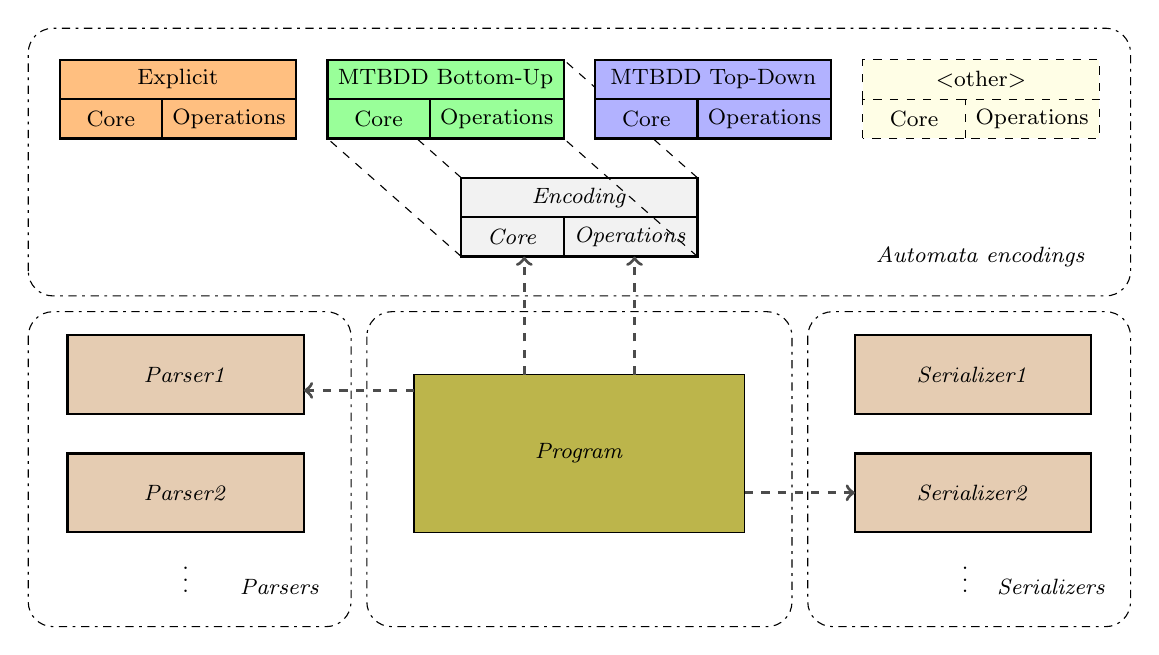
\begin{tikzpicture}
[
  scale=1,
  transform shape,
	gen/.style={thick,fill=gray!10},
	expl/.style={thick,fill=orange!50},
	bu/.style={thick,fill=green!40},
	td/.style={thick,fill=blue!30},
	other/.style={fill=yellow!10,dashed}
]
\tikzstyle{every node}=[font=\footnotesize]


% encodings
\draw[dashed] (0,1) -- (-1.7,2.5);
\draw[dashed] (0,0) -- (-1.7,1.5);
\draw[dashed] (3,1) -- (1.3,2.5);

\draw (0,0.5) rectangle +(3, 0.5) [gen] node[midway] {\textit{Encoding}};
\draw (0,0) rectangle +(1.3, 0.5) [gen] node[midway] {\textit{Core}};
\draw (1.3,0) rectangle +(1.7, 0.5) [gen] node[midway] {\textit{Operations}};

\draw (-5.1,2) rectangle +(3, 0.5) [expl] node[midway] {Explicit};
\draw (-5.1,1.5) rectangle +(1.3, 0.5) [expl] node[midway] {Core};
\draw (-3.8,1.5) rectangle +(1.7, 0.5) [expl] node[midway] {Operations};

\draw (-1.7,2) rectangle +(3, 0.5) [bu] node[midway] {MTBDD Bottom-Up};
\draw (-1.7,1.5) rectangle +(1.3, 0.5) [bu] node[midway] {Core};
\draw (-0.4,1.5) rectangle +(1.7, 0.5) [bu] node[midway] {Operations};

\draw (1.7,2) rectangle +(3, 0.5) [td] node[midway] {MTBDD Top-Down};
\draw (1.7,1.5) rectangle +(1.3, 0.5) [td] node[midway] {Core};
\draw (3.0,1.5) rectangle +(1.7, 0.5) [td] node[midway] {Operations};

\draw (5.1,2) rectangle +(3, 0.5) [other] node[midway] {$<$other$>$};
\draw (5.1,1.5) rectangle +(1.3, 0.5) [other] node[midway] {Core};
\draw (6.4,1.5) rectangle +(1.7, 0.5) [other] node[midway] {Operations};

\draw[dashed] (3,0) -- (1.3,1.5);

\draw[rounded corners=9,dash pattern=on 3pt off 2pt on 1pt off 2pt] (-5.5,-0.5) rectangle +(14,3.4);

\draw (6.6,0) node {\textit{Automata encodings}};


% parsers
\draw (-5,-2) rectangle +(3, 1) [gen,fill=brown!40] node[midway] (parser1) {\textit{Parser1}};
\draw (-5,-3.5) rectangle +(3, 1) [gen,fill=brown!40] node[midway] {\textit{Parser2}};
\draw (-3.5,-4) node {$\vdots$};

\draw[rounded corners=9,dash pattern=on 3pt off 2pt on 1pt off 2pt] (-5.5,-0.7) rectangle +(4.1,-4);
\draw (-2.3,-4.2) node {\textit{Parsers}};

% serializers
\draw (5,-2) rectangle +(3, 1) [gen,fill=brown!40] node[midway] {\textit{Serializer1}};
\draw (5,-3.5) rectangle +(3, 1) [gen,fill=brown!40] node[midway] {\textit{Serializer2}};
\draw (6.4,-4) node {$\vdots$};

\draw[rounded corners=9,dash pattern=on 3pt off 2pt on 1pt off 2pt] (4.4,-0.7) rectangle +(4.1,-4);
\draw (7.5,-4.2) node {\textit{Serializers}};

% program
\draw[rounded corners=9,dash pattern=on 3pt off 2pt on 1pt off 2pt] (-1.2,-0.7) rectangle +(5.4,-4);

\draw[fill=olive!60] (-0.6,-1.5) rectangle (3.6,-3.5) node[midway] {\textit{Program}};

\draw[very thick,dashed,->,black!70] (-0.6,-1.7) -- (-2,-1.7);
\draw[very thick,dashed,->,black!70] (3.6,-3) -- (5,-3);
\draw[very thick,dashed,->,black!70] (0.8,-1.5) -- (0.8,0);
\draw[very thick,dashed,->,black!70] (2.2,-1.5) -- (2.2,0);

\end{tikzpicture}

		\caption{The VATA library design. The image is taken from \cite{libvata}}.
		\label{picVataDesign}
\end{center}
\end{figure}

%%TODO: Vic se rozkecat o kodovanich
\subsubsection{Explicit Encoding}
\label{sectionExplicitEnc}
The explicit encoding supports storing the transitions in the top-down direction (transitions are in the form $q \xrightarrow{a} (q_1,...,q_n)$). The transitions
are stored in a \emph{hierarchical data structure based on hash tables}. The first level of the data structure is a hash table
that maps states to \emph{transition clusters}. These clusters are also look-up tables and map symbols of an input alphabet
to sets of pointers (stored as \emph{red-black trees}) to tuples of states. Storing tuples of states can be very memory demanding, so each tuple is stored
only once and is referenced by different transitions. 
Inserting a new transition to this structure requires a constant number of steps (exception is the worst case scenario) %TODO: dodelat
\cite{libvata}. This data structure can be seen in Figure \ref{figExplicitTreeDataStr}.

\begin{figure}
\begin{center}
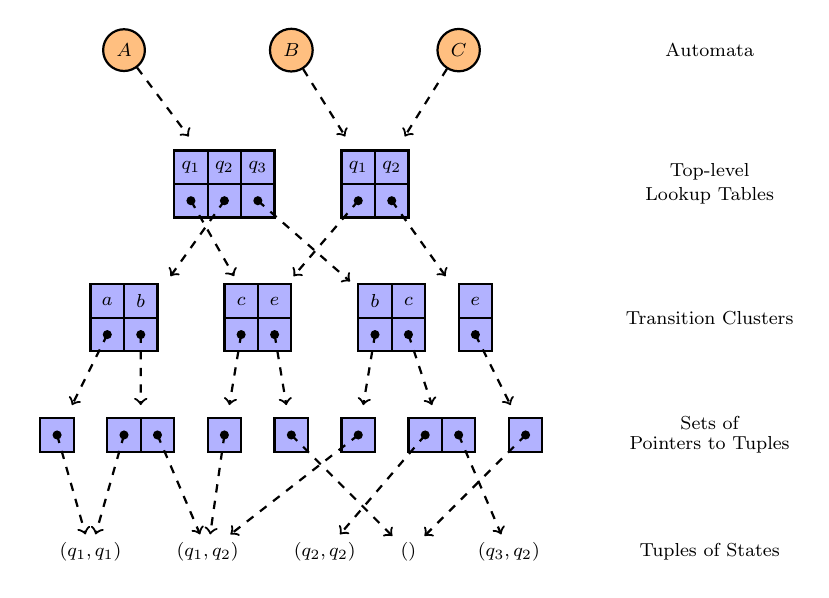
\begin{tikzpicture}
[
  scale=0.85,
  transform shape,
	gen/.style={thick,fill=gray!10},
	expl/.style={thick,fill=orange!50},
	bu/.style={thick,fill=green!40},
	td/.style={thick,fill=blue!30},
	other/.style={fill=yellow!10,dashed}
]

\node at(10,2) {Automata};

\node[expl,circle,draw] (aA) at(1.25,2) {\textit{$A$}};
\node[expl,circle,draw] (aB) at(3.75,2) {\textit{$B$}};
\node[expl,circle,draw] (aC) at(6.25,2) {\textit{$C$}};


\node at(10,0) {\shortstack{Top-level\\ Lookup Tables}};

\node[minimum size=40pt](table1) at (2.75,0) {};
\draw (2,0) rectangle +(0.5, .5) [td] node[midway] {\textit{$q_1$}};
\draw (2,-.5) rectangle +(0.5, .5) [td] node[midway] {};
\draw (2.5,0) rectangle +(0.5, .5) [td] node[midway] {\textit{$q_2$}};
\draw (2.5,-.5) rectangle +(0.5, .5) [td] node[midway] {};
\draw (3,0) rectangle +(0.5, .5) [td] node[midway] {\textit{$q_3$}};
\draw (3,-.5) rectangle +(0.5, .5) [td] node[midway] {};

\node[minimum size=40pt](table2) at (5,0) {};
\draw (4.5,0) rectangle +(0.5, .5) [td] node[midway] {\textit{$q_1$}};
\draw (4.5,-.5) rectangle +(0.5, .5) [td] node[midway] {};
\draw (5,0) rectangle +(0.5, .5) [td] node[midway] {\textit{$q_2$}};
\draw (5,-.5) rectangle +(0.5, .5) [td] node[midway] {};


\draw[->,thick,dashed] (aA) -- (table1);
\draw[->,thick,dashed] (aB) -- (table2);
\draw[->,thick,dashed] (aC) -- (table2);


\node at(10,-2) {Transition Clusters};

\node[minimum size=35](cluster1) at (1.5,-2) {};
\draw (0.75,-2) rectangle +(0.5, .5) [td] node[midway] {\textit{$a$}};
\draw (0.75,-2.5) rectangle +(0.5, .5) [td] node[midway] {};
\draw (1.25,-2) rectangle +(0.5, .5) [td] node[midway] {\textit{$b$}};
\draw (1.25,-2.5) rectangle +(0.5, .5) [td] node[midway] {};

\node[minimum size=35pt](cluster2) at (3.25,-2) {};
\draw (2.75,-2) rectangle +(0.5, .5) [td] node[midway] {\textit{$c$}};
\draw (2.75,-2.5) rectangle +(0.5, .5) [td] node[midway] {};
\draw (3.25,-2) rectangle +(0.5, .5) [td] node[midway] {\textit{$e$}};
\draw (3.25,-2.5) rectangle +(0.5, .5) [td] node[midway] {};

\node[minimum size=35pt](cluster3) at (5.25,-2) {};
\draw (4.75,-2) rectangle +(0.5, .5) [td] node[midway] {\textit{$b$}};
\draw (4.75,-2.5) rectangle +(0.5, .5) [td] node[midway] {};
\draw (5.25,-2) rectangle +(0.5, .5) [td] node[midway] {\textit{$c$}};
\draw (5.25,-2.5) rectangle +(0.5, .5) [td] node[midway] {};

\node[minimum size=35pt](cluster4) at (6.5,-2) {};
\draw (6.25,-2) rectangle +(0.5, .5) [td] node[midway] {\textit{$e$}};
\draw (6.25,-2.5) rectangle +(0.5, .5) [td] node[midway] {};


\draw[thick,fill=black] (2.25,-0.25) circle (0.5mm);
\draw[->,thick,dashed] (2.25,-.25) -- (cluster2);

\draw[thick,fill=black] (2.75,-0.25) circle (0.5mm);
\draw[->,thick,dashed] (2.75,-.25) -- (cluster1);

\draw[thick,fill=black] (3.25,-0.25) circle (0.5mm);
\draw[->,thick,dashed] (3.25,-.25) -- (cluster3);

\draw[thick,fill=black] (4.75,-0.25) circle (0.5mm);
\draw[->,thick,dashed] (4.75,-.25) -- (cluster2);

\draw[thick,fill=black] (5.25,-0.25) circle (0.5mm);
\draw[->,thick,dashed] (5.25,-.25) -- (cluster4);


\node at(10,-3.75) {\shortstack{Sets of\\ Pointers to Tuples}};

\node[minimum size=25pt](set1) at (0.25,-3.75) {};
\draw (0,-4) rectangle +(0.5, .5) [td] node[midway] {};

\node[minimum size=25pt](set2) at (1.5,-3.75) {};
\draw (1,-4) rectangle +(0.5, .5) [td] node[midway] {};
\draw (1.5,-4) rectangle +(0.5, .5) [td] node[midway] {};

\node[minimum size=25pt](set3) at (2.75,-3.75) {};
\draw (2.5,-4) rectangle +(0.5, .5) [td] node[midway] {};

\node[minimum size=25pt](set4) at (3.75,-3.75) {};
\draw (3.5,-4) rectangle +(0.5, .5) [td] node[midway] {};

\node[minimum size=25pt](set5) at (4.75,-3.75) {};
\draw (4.5,-4) rectangle +(0.5, .5) [td] node[midway] {};

\node[minimum size=25pt](set6) at (6,-3.75) {};
\draw (5.5,-4) rectangle +(0.5, .5) [td] node[midway] {};
\draw (6,-4) rectangle +(0.5, .5) [td] node[midway] {};

\node[minimum size=25pt](set7) at (7.25,-3.75) {};
\draw (7,-4) rectangle +(0.5, .5) [td] node[midway] {};


\draw[thick,fill=black] (1,-2.25) circle (0.5mm);
\draw[->,thick,dashed] (1,-2.25) -- (set1);

\draw[thick,fill=black] (1.5,-2.25) circle (0.5mm);
\draw[->,thick,dashed] (1.5,-2.25) -- (set2);

\draw[thick,fill=black] (3,-2.25) circle (0.5mm);
\draw[->,thick,dashed] (3,-2.25) -- (set3);

\draw[thick,fill=black] (3.5,-2.25) circle (0.5mm);
\draw[->,thick,dashed] (3.5,-2.25) -- (set4);

\draw[thick,fill=black] (5,-2.25) circle (0.5mm);
\draw[->,thick,dashed] (5,-2.25) -- (set5);

\draw[thick,fill=black] (5.5,-2.25) circle (0.5mm);
\draw[->,thick,dashed] (5.5,-2.25) -- (set6);

\draw[thick,fill=black] (6.5,-2.25) circle (0.5mm);
\draw[->,thick,dashed] (6.5,-2.25) -- (set7);


\node at(10,-5.5) {Tuples of States};

\node(tup1) at (0.75,-5.5) {$(q_1, q_1)$};
\node(tup2) at (2.5,-5.5) {$(q_1, q_2)$};
\node(tup3) at (4.25,-5.5) {$(q_2, q_2)$};
\node(tup4) at (7,-5.5) {$(q_3, q_2)$};
\node(tup5) at (5.5,-5.5) {$()$};

\draw[thick,fill=black] (0.25,-3.75) circle (0.5mm);
\draw[->,thick,dashed] (0.25,-3.75) -- (tup1);

\draw[thick,fill=black] (1.25,-3.75) circle (0.5mm);
\draw[->,thick,dashed] (1.25,-3.75) -- (tup1);

\draw[thick,fill=black] (1.75,-3.75) circle (0.5mm);
\draw[->,thick,dashed] (1.75,-3.75) -- (tup2);

\draw[thick,fill=black] (2.75,-3.75) circle (0.5mm);
\draw[->,thick,dashed] (2.75,-3.75) -- (tup2);

\draw[thick,fill=black] (3.75,-3.75) circle (0.5mm);
\draw[->,thick,dashed] (3.75,-3.75) -- (tup5);

\draw[thick,fill=black] (4.75,-3.75) circle (0.5mm);
\draw[->,thick,dashed] (4.75,-3.75) -- (tup2);

\draw[thick,fill=black] (5.75,-3.75) circle (0.5mm);
\draw[->,thick,dashed] (5.75,-3.75) -- (tup3);

\draw[thick,fill=black] (6.25,-3.75) circle (0.5mm);
\draw[->,thick,dashed] (6.25,-3.75) -- (tup4);

\draw[thick,fill=black] (7.25,-3.75) circle (0.5mm);
\draw[->,thick,dashed] (7.25,-3.75) -- (tup5);


\end{tikzpicture}

    \caption{The data structure for storing transitions of the tree automaton. There is a hash table (top-level look-up table) 
      which map a state to the pointer to another hash table (transition cluster). Transition cluster
      maps a symbols of input alphabet to the pointer to the set of pointers to the tuples of states.}
		\label{figExplicitTreeDataStr}
\end{center}
\end{figure}


For better performance the \emph{copy-on-write} technique \cite{libvata} is used. The principle of this technique is 
that copying an automaton creates just a new pointer to the transition table of original automaton and after adding a new state to one of the automata 
only a part of the whole shared transition table is modified. 

\subsubsection{Semi-symbolic Encoding}
Transition functions in the semi-symbolic encoding are stored in \emph{multi-terminal binary decision diagrams} (MTBDD), 
which are extension of \emph{binary decision 
diagrams}. Two representations of tree automata are provided in the semi-symbolic encoding: top-down and bottom-up. 
The specific part is the saving of symbols into a MTBDD. In the top-down representation, the input
symbols are stored in the MTBDD with their arity, because we need to be able to distinguish between two instances of the same symbols with a different arity.
In the opposite case, the bottom-up representation does not need to store the arity, because it is possible to get it from the arity of tuples 
on the left-hand side of transition \cite{libvata}.

For the purposes of the VATA library a new MTBDD package was implemented which improves the performance of the library.

\subsubsection{Operations}
There are several supported basic operations over tree automata 
such as union, intersection, elimination of unreachable states, but also some advanced algorithms for inclusion checking, 
computation of the simulation relation, language preserving size reduction based on the simulation equivalence. 

Optimized algorithms for inclusion testing based on the algorithms from \cite{cav06,tacas10} are implemented. 
The inclusion test is implemented in more versions, so it is possible
to use only some heuristics and compare different results.

The efficiency of the advanced operations does not come only from the usage of the state-of-the-art algorithms, 
but there are also some implementation optimizations like the \emph{copy-on-write}
principle for automata copying (briefly described in Section \ref{sectionExplicitEnc}), buffering already computed clusters of transitions, etc. 
Other optimizations could be found in exploitation of polymorphism using C++ function templates, instead of
virtual methods because a call of a virtual function leads to an indirect function call using look-up in a virtual method table 
(because the compiler does not know in advance which function will be called in runtime), which brings an overhead compared to the classical direct 
function call and it also precludes compiler's optimizer to perform some optimization. 
More details about implementation optimization can be found in \cite{libvata}.

Especially advanced operations are implemented only for a specific encoding. Some of the operations implemented in the VATA library and their 
supported encodings are in Table \ref{tabOp}.
\begin{savenotes}
\begin{table}[h]
	\begin{center}
		\catcode`\-=12
		\begin{tabular}{| l | c | c | c |} \hline
		& {\textbf{Explicit}} & \multicolumn{2}{|c|}{\textbf{Semi-symbolic}} \\ \cline{2-4}
		\textbf{Operation} & \textbf{top-down} & \textbf{bottom-up} & \textbf{top-down} \\ \hline
		Union & $+$ & $+$ & $+$ \\
		Intersection & $+$ & $+$ & $+$ \\
		Complement & $+$ & $-$ & $-$ \\
		Removing useless states & $+$ & $+$ & $+$ \\
		Removing unreachable states & $+$ & $+$ & $+$ \\
		Downward Simulation & $+$ & $+$ & $+$ \\
		Upward Simulation & $+$ & $-$ & $+$ \\
		Bottom-Up Inclusion  & $+$ & $+$ & $-$ \\ 
    \hline
		\end{tabular}
	\caption{Table shows which operations are supported for the tree automata in the encodings implemented in the VATA library.}
	\label{tabOp}
	\end{center}
\end{table}
\end{savenotes}


\subsection{Extension for Finite Automata}
The purposes of the VATA library are similar as purposes of this work and because the VATA library is written in a modular way, it is easy 
to extend it by another module. It was therefore decided not to create a brand new library but implement new extension of VATA for finite automata.

The main goal is to provide an efficient implementation of the operation of checking language inclusion using state-of-the-art algorithms. 
To be precise the VATA library can be already used for finite automata which can be represented by unary
tree automata. But the VATA library data structures for manipulating tree automata are designated for more complex data structures
and new special implementation for finite automata will be definitely more efficient. 
Not only inclusion checking algorithms will be implemented, but also algorithms for basic operations like union, intersection and removing unreachable or 
useless states. The new extension will implement only the explicit encoding of finite automata. 
The extension will use some already implemented features of the VATA library like the parser and the serializer 
or computation of simulation over states of an automaton.

\chapter{Design}
\label{design}
This chapter is primarily about the design of the newly created extension of the VATA library for finite automata. 
At first, the data structures used for storing a finite automaton will be described, then a principle of the translation of the states and the symbols of an NFA 
to the internal representation. The choice of the input format and its modification are justified.  
The algorithms for basic operations over NFA such as union, intersection or removing unreachable states, etc., are given at the end of the chapter.

\section{Data Structures for Explicit Encoding of Finite Automata}
The encodings for tree automata used in the VATA library differ mainly in the data structure used for storing transitions of tree automata. The explicit encoding
for finite automata is defined by a data structure used for storing the transitions too. 
This data structure is also crucial for the performance of the algorithms so it is important to take care when analyzing and designing it. 

\label{data structure explicit}
\subsection{Analysis}
\label{analysis}
A NFA is defined by the set of its states, its initial and final states (which are subsets of the set of all states of the NFA) and also its
transitions and the input alphabet (a formal definition is given in Section \ref{defNFA}). 
One needs to keep information about sets of initial and final states to be able to distinguish
between them and the other states. However it is not necessary to store the whole set of states itself because it is given implicitly by the states used 
inside transitions. This also holds for the input alphabet of the NFA. 

The transitions keep the most information about an NFA and are also often used
during the operations over the NFA, so the performance of these operations strongly depend on the efficiency of the data structure used to store transitions. 
For an example, in many operations over the NFA one wants to get all transitions for a given state and a given alphabet symbol and it is important for 
the efficiency of the algorithms to get those transitions in as few steps as possible. The similar needs are in the case
of tree automata when it is not necessary to hold the whole set of the states but it is important to have an efficient data structure for representing 
transitions of the tree automaton.

The data structure used for storing transitions of a tree automaton in the VATA library was described earlier in Section \ref{sectionExplicitEnc} and can be seen
in Figure \ref{figExplicitTreeDataStr}. The evaluation of the VATA library \cite{libvata} proves the efficiency of this data structure so it was
decided to modify it and implement its modification also in the extension of the VATA library for finite automata.

\subsection{Design of Data Structure for Transitions of NFA}
The data structure for storing transitions of an NFA is based on hash tables. The first hash table (top-level hash table) maps a given state to the pointer to
a transition cluster. The transition cluster is another hash table which maps a given symbol of the input alphabet to a set of states accessible from
the given state under the given symbol. 
The described data structure is in figure \ref{figExplicitFADataStr}.

The data structure for storing transitions of an NFA is a simplification of the data structure for tree automata. Since transitions of a tree automaton
has the following form: $q \xrightarrow{a} (q_1,\ldots,q_n)$ where $q,q_1\ldots q_n$ are states of the tree automaton and $a$ is a symbol of 
the input alphabet of the tree automaton, and a finite automaton has transitions of the form: $q_1 \xrightarrow{a} q_2$ 
where $q_1,q_2$ are states of the finite automaton and $a$ is a symbol of its alphabet, the simplification of the data structure is possible because 
the tree version has to store the whole tuples. These tuples can be very large and it is more efficient to store them only once in a cache and 
in the data structure for transitions work only with a pointer to a tuple instead of the tuple itself. 

In the case of finite automata this advantage disappears because there are no tuples of state but only states alone and keeping a pointer to one state
would only bring unnecessary overhead 
(a size of a pointer to a state is usually equal or bigger than the state represented by an integer). This causes that it is not needed 
for the data structure for finite automata to use 
anything such as a set of pointers to tuples, but a set of states could be directly used instead of
a set of pointers. The set of states would be referenced from transition clusters and would contain all states accessible from a given state under a 
certain symbol of the input alphabet.

But there is another possible simplification. The set of states does not need to be in a special set referenced by transition clusters but can be integrated
into the transition cluster. When this optimization is applied, the transition cluster maps a symbol directly to the set of states accessible under this symbol.

The mentioned optimization enables simplification from the four levels of the data structure for tree automata to the two levels of the
data structure used for finite automata which, 
brings simpler and more efficient manipulation with these data structure. A comparison of the data structure for finite automata and 
tree automata can be seen in Figure \ref{figExplicitFADataStr} and Figure \ref{figExplicitTreeDataStr}.

This data structure also applies the copy-on-write principle for better memory efficiency so the look-up tables and 
the transition clusters are shared among NFA when they are the same and
a new look-up table and a transition is created only when a new item is inserted to one of the automata. For example, NFA $\mathcal{B}$ and NFA $\mathcal{C}$
in Figure \ref{figExplicitFADataStr} are sharing the same data structure.

Let us give examples for searching and inserting a transition into this data structure for the NFA in Figure \ref{figExplicitFADataStr}. 
If one wants to find all accessible states from the state $q_1$ over the symbol $a$ in an NFA $\mathcal{A}$.
First, the transition cluster that corresponds to $q_1$ is found in the top-level look-up table and then the set of states mapped by $a$ is retrieved if there
is such.
If one wants to insert a new transition $q_3 \xrightarrow{e} q_2$ to an NFA $\mathcal{C}$, the look-up table for automaton $\mathcal{C}$ is duplicated
because $\mathcal{C}$ has been sharing the look-up table with automaton $\mathcal{B}$,
and finally a state $q_3$ is inserted into it. The NFA $\mathcal{C}$ now points to that newly duplicated look-up table. State $q_3$ is in this look-up table 
mapped to a pointer to the newly created transition cluster. 
The symbol $e$ is inserted to this new transition cluster and mapped to the set of states which contains only the state $q_2$.

\begin{figure}[bt]
\begin{center}
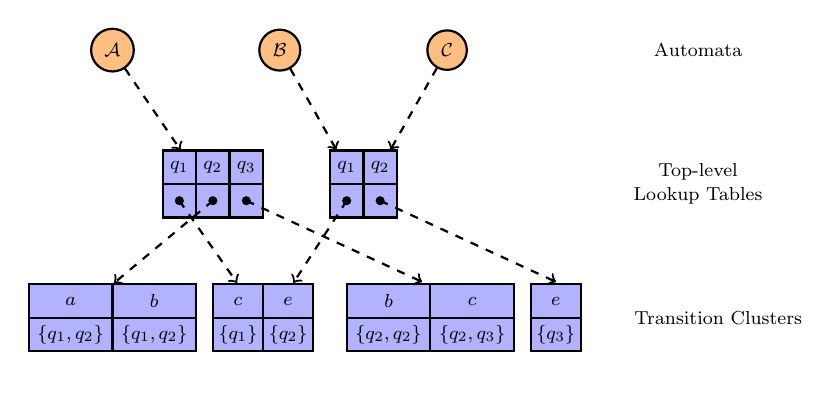
\begin{tikzpicture}
[
  scale=0.85,
  transform shape,
	gen/.style={thick,fill=gray!10},
	expl/.style={thick,fill=orange!50},
	bu/.style={thick,fill=green!40},
	td/.style={thick,fill=blue!30},
	other/.style={fill=yellow!10,dashed}
]

\node at(10,2) {Automata};

\node[expl,circle,draw] (aA) at(1.25,2) {\textit{$\mathcal{A}$}};
\node[expl,circle,draw] (aB) at(3.75,2) {\textit{$\mathcal{B}$}};
\node[expl,circle,draw] (aC) at(6.25,2) {\textit{$\mathcal{C}$}};


\node at(10,0) {\shortstack{Top-level\\ Lookup Tables}};

\node[minimum size=40pt](table1) at (2.75,-0.2) {};
\draw (2,0) rectangle +(0.5, .5) [td] node[midway] {\textit{$q_1$}};
\draw (2,-.5) rectangle +(0.5, .5) [td] node[midway] {};
\draw (2.5,0) rectangle +(0.5, .5) [td] node[midway] {\textit{$q_2$}};
\draw (2.5,-.5) rectangle +(0.5, .5) [td] node[midway] {};
\draw (3,0) rectangle +(0.5, .5) [td] node[midway] {\textit{$q_3$}};
\draw (3,-.5) rectangle +(0.5, .5) [td] node[midway] {};

\node[minimum size=40pt](table2) at (5,-0.2) {};
\draw (4.5,0) rectangle +(0.5, .5) [td] node[midway] {\textit{$q_1$}};
\draw (4.5,-.5) rectangle +(0.5, .5) [td] node[midway] {};
\draw (5,0) rectangle +(0.5, .5) [td] node[midway] {\textit{$q_2$}};
\draw (5,-.5) rectangle +(0.5, .5) [td] node[midway] {};


\draw[->,thick,dashed] (aA) -- (table1);
\draw[->,thick,dashed] (aB) -- (table2);
\draw[->,thick,dashed] (aC) -- (table2);


\node at(10.3,-2) {Transition Clusters};

\node[minimum size=35](cluster1) at (0.65,-2) {};
\draw (0.00,-2) rectangle +(1.25, .5) [td] node[midway] {\textit{$a$}};
\draw (0.00,-2.5) rectangle +(1.25, .5) [td] node[midway] {\textit{$\{q_1,q_2\}$}};
\draw (1.25,-2) rectangle +(1.25, .5) [td] node[midway] {\textit{$b$}};
\draw (1.25,-2.5) rectangle +(1.25, .5) [td] node[midway] {\textit{$\{q_1,q_2\}$}};

\node[minimum size=35pt](cluster2) at (3.55,-2.1) {};
\draw (2.75,-2) rectangle +(0.75, .5) [td] node[midway] {\textit{$c$}};
\draw (2.75,-2.5) rectangle +(0.75, .5) [td] node[midway] {\textit{$\{q_1\}$}};
\draw (3.5,-2) rectangle +(0.75, .5) [td] node[midway] {\textit{$e$}};
\draw (3.5,-2.5) rectangle +(0.75, .5) [td] node[midway] {\textit{$\{q_2\}$}};

\node[minimum size=35pt](cluster3) at (6.5,-1.75) {};
\draw (4.75,-2) rectangle +(1.25, .5) [td] node[midway] {\textit{$b$}};
\draw (4.75,-2.5) rectangle +(1.25, .5) [td] node[midway] {\textit{$\{q_2,q_2\}$}};
\draw (6.0,-2) rectangle +(1.25, .5) [td] node[midway] {\textit{$c$}};
\draw (6.0,-2.5) rectangle +(1.25, .5) [td] node[midway] {\textit{$\{q_2,q_3\}$}};

\node[minimum size=35pt](cluster4) at (8.5,-1.75) {};
\draw (7.5,-2) rectangle +(0.75, .5) [td] node[midway] {\textit{$e$}};
\draw (7.5,-2.5) rectangle +(0.75, .5) [td] node[midway] {\textit{$\{q_3\}$}};


\draw[thick,fill=black] (2.25,-0.25) circle (0.5mm);
\draw[->,thick,dashed] (2.25,-.25) -- (cluster2);

\draw[thick,fill=black] (2.75,-0.25) circle (0.5mm);
\draw[->,thick,dashed] (2.75,-.25) -- (cluster1);

\draw[thick,fill=black] (3.25,-0.25) circle (0.5mm);
\draw[->,thick,dashed] (3.25,-.25) -- (cluster3);

\draw[thick,fill=black] (4.75,-0.25) circle (0.5mm);
\draw[->,thick,dashed] (4.75,-.25) -- (cluster2);

\draw[thick,fill=black] (5.25,-0.25) circle (0.5mm);
\draw[->,thick,dashed] (5.25,-.25) -- (cluster4);
\end{tikzpicture}

    \caption{The data structure for storing transitions of an NFA. There is a hash table (top-level look-up table) 
      which maps a state of an NFA to the pointer to another hash table (transition cluster). The transition cluster maps symbols of the input alphabet
      to sets of states.}
		\label{figExplicitFADataStr}
\end{center}
\end{figure}

\section{Data Structure for Initial and Final States}
As it was mentioned in the previous section it is necessary to keep initial and final states in special sets to 
be able distinguish between them and the other states of an automaton. This is also the main use of these sets during operations 
over finite automata so there is no need to create a special data structure and a hash table is efficient enough for this purposes. %TODO: popsat detailneji

\section{Translation of the States and Symbols}
\label{sectionTranslate}
An automaton is always parsed and converted to the internal representation from its input format. 
The conversion to the internal representation is based on mapping states from an input type (e.g. text description of the automaton) 
to integers. This principle is also applied for symbols of the input alphabet. 
The mechanism of translation is illustrated in figure~\ref{figExplicitFATransl}. 
The mechanism brings better efficiency for manipulation with states and symbols
during the operations. It also provides unification of all input forms to the one internal representation. 

Execution of some operations (e.g., union) can causes reindexing of the states, which means that the integers 
which represent states are changed. When the integer is changed an old value is mapped to a new one by a hash table that keeps 
relation between the original input value and the new integer value.

When the operations over an NFA are performed it may be desirable to serialize the output NFA. The states and symbols of the resulting
automaton are mapped back to the input notation using hash tables where the mapping has been stored. This
principle brings more readable output of serialization because the original notation is kept (if it is possible).

\begin{figure}[bt]
\begin{center}
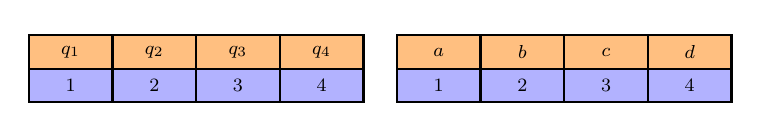
\begin{tikzpicture}
[
  scale=0.85,
  transform shape,
	gen/.style={thick,fill=gray!10},
	expl/.style={thick,fill=orange!50},
	bu/.style={thick,fill=green!40},
	td/.style={thick,fill=blue!30},
	other/.style={fill=yellow!10,dashed}
]

\node[minimum size=35](states) at (0.65,-2) {};
\draw (0.00,-2) rectangle +(1.25, .5) [expl] node[midway] {\textit{$q_1$}};
\draw (0.00,-2.5) rectangle +(1.25, .5) [td] node[midway] {\textit{$1$}};
\draw (1.25,-2) rectangle +(1.25, .5) [expl] node[midway] {\textit{$q_2$}};
\draw (1.25,-2.5) rectangle +(1.25, .5) [td] node[midway] {\textit{$2$}};
\draw (2.5,-2) rectangle +(1.25, .5) [expl] node[midway] {\textit{$q_3$}};
\draw (2.5,-2.5) rectangle +(1.25, .5) [td] node[midway] {\textit{$3$}};
\draw (3.75,-2) rectangle +(1.25, .5) [expl] node[midway] {\textit{$q_4$}};
\draw (3.75,-2.5) rectangle +(1.25, .5) [td] node[midway] {\textit{$4$}};

\node[minimum size=35](syms) at (0.65,-2) {};
\draw (5.5,-2) rectangle +(1.25, .5) [expl] node[midway] {\textit{$a$}};
\draw (5.5,-2.5) rectangle +(1.25, .5) [td] node[midway] {\textit{$1$}};
\draw (6.75,-2) rectangle +(1.25, .5) [expl] node[midway] {\textit{$b$}};
\draw (6.75,-2.5) rectangle +(1.25, .5) [td] node[midway] {\textit{$2$}};
\draw (8.0,-2) rectangle +(1.25, .5) [expl] node[midway] {\textit{$c$}};
\draw (8.0,-2.5) rectangle +(1.25, .5) [td] node[midway] {\textit{$3$}};
\draw (9.25,-2) rectangle +(1.25, .5) [expl] node[midway] {\textit{$d$}};
\draw (9.25,-2.5) rectangle +(1.25, .5) [td] node[midway] {\textit{$4$}};

\end{tikzpicture}

    \caption{The figure shows a principle of the translation of the input format to the internal representation by a hash table. 
      The states (the left hash table) or of the symbols (the right hash table) of a NFA are mapped from strings to the integers.}
		\label{figExplicitFATransl}
\end{center}
\end{figure}

\section{Use of the Timbuk Format}
\label{usageTimbuk}
The VATA library provides the possibility to load a finite automaton from a text specification. 
The text specification of NFA has to have a standard format but there is no such format for the finite automata so
a modification of the Timbuk format was chosen \cite{timbuk}. 
The Timbuk format is primarily used for the description of tree automata but can be also used for finite automata
after some modifications. This format is also used as the input format of tree automata in the VATA library.

An example of a finite automaton defined by text description in the Timbuk format is given in Figure \ref{figTimbukFormat}.
\begin{figure}[bt]
\begin{center}
\texttt {
  \begin{packed_enum}
  \item \textbf{Ops} $a:1$ $x:0$\\
  \item \textbf{Automaton} foo\\
  \item \textbf{States} $s$ $p$ $q$ $f$\\
  \item \textbf{Final States} $f$\\
  \item \textbf{Transitions}\\
  \item \indent $x \rightarrow s$\\
  \item \indent $a(s) \rightarrow p$\\
  \item \indent $a(s) \rightarrow q$\\
  \item \indent $a(p) \rightarrow f$\\
  \item \indent $a(q) \rightarrow f$\\
  \end{packed_enum}
}
\caption{An NFA defined by text description in the Timbuk format}
\label{figTimbukFormat}
\end{center}
\end{figure}
On the first line in Figure \ref{figTimbukFormat} of the specification in the Timbuk format
it is specified that the automaton has only one symbol of the input alphabet $a$ with arity one (arity of the symbols of finite automata will
be always one). 
The need to specify of the arity of an input symbol is a necessity which comes from the original purpose of the Timbuk format because it is necessary 
to give the arity of a symbol of the input alphabet of the tree automaton.

The second symbol $x$ with arity zero is not actually a symbol of the input alphabet but is used for definition of the initial states. The
initial states are defined in the part \emph{Transitions} by the transitions which has on the left-hand side a symbol with zero arity; the
right-hand side of the transition defines a initial state. This is again a disadvantage
of the Timbuk format because tree automata have no initial states.

On the second line in Figure \ref{figTimbukFormat} is the name of the automaton (our example the name is \emph{foo}). 
On the third line is a list of states of the automaton and on the fourth line is a list of final states of the automaton.
Then there is a list of transitions of the automaton. 
For example, the transition $s \xrightarrow{a} q$ is in the Timbuk format described as $a(s)\rightarrow q$.

\section{Algorithms for Basic Operations}
In this section we describe algorithms used for implementation of basic operations, such as union, intersection or removing useless states. 

\subsection{Union}
The union of two NFA $\mathcal{A}$ and $\mathcal{B}$ is described in section \ref{defAUnion} and
is done by the following algorithm. First, a brand new automaton is created (this automaton
will be the result of the operation). 
Sets of initial and final states are copied to this automaton from both original automata. Then all transitions from $\mathcal{A}$ and
$\mathcal{B}$ are added to the newly created automaton. What is the most important part during the previous operations is reindexing of states. 
The reindexing means that we create an index which maps
integers that represent states in the input automaton to new integers representing the same state in the automaton created by this union.

The reindexing of states is done because the same integer can be used for representing one state of a NFA $\mathcal{A}$ 
and also another state of a NFA $\mathcal{B}$ and it is important
to be able to distinguish between these two states in the result NFA. This technique also makes text output of serialization of the result automaton 
more readable because its states have the same names as they have in the input automata, only indices $1$ and $2$ are added in order to be able to 
distinguish between states of both automata. E.g., a state $q$ of the NFA $\mathcal{A}$ and a state $q$ of the 
NFA $\mathcal{B}$ are in the result automaton denoted as $q_1$ and $q_2$.

\subsubsection{Union of NFAs with Disjoint Sets of States}
The special case of a union of two NFA is a union when states of these NFA have disjunct sets of states. 
This is done by copying the first NFA to the result automaton and then
the states (and transitions which contain these states) of the second NFA which are not already in the result NFA are copied to the result automaton.
No reindexing of states is done during this operation.

\subsection{Intersection}
The algorithm for computing the intersection automaton for two NFA $\mathcal{A}=(Q_\mathcal{A},\Sigma,\delta_\mathcal{A},I_\mathcal{A},F_\mathcal{A})$
and $\mathcal{B}=(Q_\mathcal{A},\Sigma,\delta_\mathcal{B},I_\mathcal{B},F_\mathcal{B})$ was introduced 
in Section \ref{defAInter}. 
We define the post-image of the product state $(p,q)\in \mathcal{A}\cap\mathcal{B}$ for a given symbol $a\in \Sigma$ as: 
$Post_a((p,q)):=\{(p',q')\ |\ \exists a \in \Sigma: (p,a,p')\in \delta_a, (q,a,q')\in \delta_b\}$.
The algorithm for intersection is given in Algorithm \ref{algIntersection}.

The principle of this algorithm is the following. Both input NFA are explored parallel and the product states are added into the result automaton. 
A product state consists of two states each from a different automaton which are accessible through the same word over the input alphabet. 
The transitions of the result automaton also contains these product states.

\begin{figure}[bt]
\begin{algorithm}[H]
	\label{algIntersection}
	\KwIn{NFAs $\mathcal{A}=(Q_\mathcal{A},\Sigma,\delta_\mathcal{A},I_\mathcal{A},F_\mathcal{A}),\ \mathcal{B}=(Q_\mathcal{B},\Sigma,
      \delta_\mathcal{B},I_\mathcal{B},F_\mathcal{B})$} 

  \KwOut{NFA $\mathcal{A}\cap\mathcal{B}$=($Q_{\mathcal{A}\cap\mathcal{B}},\Sigma,\delta_{\mathcal{A}\cap\mathcal{B}},
      I_{\mathcal{A}\cap\mathcal{B}},F_{\mathcal{A}\cap\mathcal{B}}$)}
  $Stack := \emptyset$\;
  $Reachable := \emptyset$\;

  \ForEach{$(p_\mathcal{A},p_\mathcal{B})\in I_\mathcal{A}\times I_\mathcal{B}$} {
    Add $(p_\mathcal{A},p_\mathcal{B})$ to $I_{\mathcal{A} \cap \mathcal{B}}$\;
    \If{$(p_\mathcal{A},p_\mathcal{B})\not\in\ Reachable$} {
      Add $(p_\mathcal{A},p_\mathcal{B})$ to $Reachable$\;
      Push $(p_\mathcal{A},p_\mathcal{B})$ on $Stack$\; 
    }
    \If{$(p_\mathcal{A} \in F_\mathcal{A} \wedge p_\mathcal{B} \in F_\mathcal{B})$} {
      Add $(p_\mathcal{A},p_\mathcal{B})$ to $F_{\mathcal{A}\cap\mathcal{B}}$
    }
  }
	
  \While{($Stack\neq \varnothing$)} {
			Pick and remove a product-state $(p_\mathcal{A},p_\mathcal{B})$ from $Stack$\;
			\ForEach{$(q_\mathcal{A},q_\mathcal{B})\in Post_a(p_\mathcal{A},p_\mathcal{B}),\forall a\in\Sigma$}{ %TODO foreach a in sigma
        \If{$(q_\mathcal{A} \in F_\mathcal{A} \wedge q_\mathcal{B} \in F_\mathcal{B})$} {
          Add $(q_\mathcal{A},q_\mathcal{B})$ to $F_{\mathcal{A}\cap\mathcal{B}}$
        }
        Add $(p_\mathcal{A},p_\mathcal{B}) \xrightarrow{a} (q_\mathcal{A},q_\mathcal{B})$ to $\delta_{\mathcal{A}\cap\mathcal{B}}$\;
        \If{$(q_\mathcal{A},q_\mathcal{B})\not\in\ Reachable$} {
           Add $(q_\mathcal{A},q_\mathcal{B})$ to $Reachable$\;
           Push $(q_\mathcal{A},q_\mathcal{B})$ on $Stack$\; 
        }
      }
	 }
		\Return NFA $\mathcal{A}\cap\mathcal{B}$=($Q_{\mathcal{A}\cap\mathcal{B}},\Sigma,\delta_{\mathcal{A}\cap\mathcal{B}},
      I_{\mathcal{A}\cap\mathcal{B}},F_{\mathcal{A}\cap\mathcal{B}}$);
	\caption{Algorithm for computing intersection of pair of NFA}
\end{algorithm}
\end{figure}

\subsection{Reversal}
The reversion of an NFA $\mathcal{A}=(Q_\mathcal{A},\Sigma,\delta_\mathcal{A},I_\mathcal{A},F_\mathcal{A})$ is the NFA 
$\mathcal{A}_{rev}=(Q_{\mathcal{A}},\Sigma,\delta_{\mathcal{A}_{rev}},F_{\mathcal{A}},I_{\mathcal{A}})$ 
which is created just by swapping the sets of initial and final states and reverting all transitions  so e.g., transition
$p\xrightarrow{x}q \in \delta_\mathcal{A}$ is added to $\delta_{\mathcal{A}_{rev}}$ in the form $q\xrightarrow{a}p$.

\subsection{Removing Unreachable States}
Let the NFA $\mathcal{B}$ be created by removing all unreachable states from an NFA $\mathcal{A}$ (an unreachable state of an NFA was defined in
section \ref{defRun}). The algorithm for removing all unreachable states implemented in the VATA library is described in Algorithm \ref{algRemove}.

The intuition behind the algorithm is following. The NFA $\mathcal{A}$ is explored from its start states and to the result automaton 
there are added only those states which are
reachable from these initial states for some word $w \in \Sigma^{*}$. At first, all reachable states are found and added to a special set. 
Then all transitions with a reachable state on left-hand side are added to the result NFA $\mathcal{B}$.
If a found reachable state is a final state of 
$\mathcal{A}$ it is also added to the set of final states of $\mathcal{B}$. A set of initial states is copied from
NFA $\mathcal{A}$ to NFA $\mathcal{B}$

\subsection{Removing Useless States}
Useless state of an NFA were defined in Section \ref{defRun}. Removing useless states from an NFA $\mathcal{A}$ is done simply by
removing all unreachable states of the NFA $\mathcal{A}$, 
then we revert NFA $\mathcal{A}$ and remove unreachable states in this reverted automaton and finally $\mathcal{A}$ is reverted back to the
originally direction. The NFA $\mathcal{A}$ does not contain any useless states after this sequence of operations.

\begin{figure}[h!]
\begin{algorithm}[H]
	\label{algRemove}
	\KwIn{NFA $\mathcal{A}=(Q_\mathcal{A},\Sigma,\delta_\mathcal{A},I_\mathcal{A},F_\mathcal{A})$} 

  \KwOut{NFA $\mathcal{B}=(Q_\mathcal{B},\Sigma,
      \delta_\mathcal{B},I_\mathcal{B},F_\mathcal{B})$}
  $Reachable := I_\mathcal{A}$\;
  $Stack := Reachable$\;
	
  \While{$Stack\neq \emptyset$} {
			Pick and remove a state $p$ from $Stack$\;
			\ForEach{$q\in Post_a(p),\forall a\in\Sigma$}{ %TODO forall a in simga
        \If{$q\in\ F_\mathcal{A}$}{
              Add $q$ to $F_\mathcal{B}$\;
        }
        Add $\{(q,a,q')\ |\ \exists a \in \Sigma, q'\in Q_\mathcal{A}: (q,a,q')\in \delta_\mathcal{A}\}$ to $\delta_\mathcal{B}$\;
        \If{$(q \not\in\ Reachable)$} {
          Push $q$ on $Stack$\;
          Add $q$ to $Reachable$\;
        }
      }
	 }

  $I_{\mathcal{B}} = I_{\mathcal{A}}$\;
	\Return NFA $\mathcal{B}=(Q_\mathcal{B},\Sigma,\delta_\mathcal{B},I_\mathcal{B},F_\mathcal{B})$;
	\caption{Algorithm for removing the unreachable states of an NFA}
\end{algorithm}
\begin{algorithm}[H]
	\label{algCandidate}
	\KwIn{NFA $\mathcal{A}=(Q_\mathcal{A},\Sigma,\delta_\mathcal{A},I_\mathcal{A},F_\mathcal{A})$} 

  \KwOut{NFA $\mathcal{B}=(Q_\mathcal{B},\Sigma,\delta_\mathcal{B},I_\mathcal{B},F_\mathcal{B})$}

  $I_\mathcal{B} := I_\mathcal{A}$\;
  $Reachable := I_\mathcal{A}$\;
  $Stack := Reachable$\;
	
  \While{$Stack\neq \varnothing$} {
			Pick and remove a state $p$ from $Stack$\;
			\ForEach{$p\xrightarrow{a}q\in\{p'\xrightarrow{a}q'\ |\ \exists a\in \Sigma:p'\xrightarrow{a}q'\in\delta_\mathcal{A}\}$}{
        \If{$(q \not\in\ Reachable)$} {
          Push $q$ on $Stack$\;
          Add $q$ to $Reachable$\;
        }
        Insert $p\xrightarrow{a}q$ to $\delta_{\mathcal{B}}$\;
        \If{$q\in\ F_\mathcal{A}$}{
          Add $q$ to $F_\mathcal{B}$\;
          Remove useless states from NFA $\mathcal{B}$
	        \Return NFA $\mathcal{B}$;
        }
      }
	}

  Remove useless states from NFA $\mathcal{B}$\;
	\Return NFA $\mathcal{B}=(Q_\mathcal{B},\Sigma,\delta_\mathcal{B},I_\mathcal{B},F_\mathcal{B})$;
	\caption{Algorithm for getting a witness in an NFA}
\end{algorithm}


\end{figure}

\subsection{Get Candidate}
The operation of a getting a word (also called get a witness) of an NFA $\mathcal{A}=(Q_\mathcal{A},\Sigma,\delta_\mathcal{A},I_\mathcal{A},F_\mathcal{A})$ 
creates an NFA $\mathcal{B}=(Q_\mathcal{B},\Sigma,\delta_\mathcal{B},I_\mathcal{B},F_\mathcal{B})$ such that language $L_\mathcal{B}$
is a subset of the language $L_\mathcal{A}$ and is non-empty iff $L_\mathcal{A}$ is non-empty too.
The NFA $\mathcal{B}$ should accept at most one word such that its length is the smallest from all words accepted by $\mathcal{A}$.

The operation for getting candidate is implemented in Algorithm \ref{algCandidate}. This algorithm copies the set of initial states 
of $\mathcal{A}$ to a set of initial states of $\mathcal{B}$ and also adds the initial states to a set of reachable states. 
Then all transitions from $\delta_\mathcal{A}$ containing on the left-hand side a state from the set of reachable states are added to $\delta_\mathcal{B}$ 
and finally
all successors of the currently reachable states are added to the set of reachable states too. 
This is repeated until final state is not accessible from any reachable state. 
%TODO udelat podle ondry

\chapter{Implementation}
\label{implementation}
This chapter provides the description of the VATA library module for finite automata. Loading of a finite
automaton to explicit encoding will be described first. 
Then a list of the used modules from the original VATA implementation is given and finally the implementation of algorithms 
for checking language inclusion is covered.

\section{Loading and Manipulation with Finite Automata in the Explicit Encoding}
Loading of an finite automaton to the explicit representation 
is done by  the class \emph{ExplicitFiniteAut} which is the main class for representation of a finite automaton. 
This class has the data members that implement the data structure for explicit encoding of a finite automaton described in Chapter \ref{design} and
implements also the copy-on-write principle. 
It is possible to load the finite automaton from a data structure returned by a parser or directly from a text specification. 
The class also provides functions for serialization of the finite automaton back to the text specification.
It implements the operations for manipulation with an automaton such as setting specific state as initial or final.
The class \emph{ExplicitFiniteAut} also ensures translation (mentioned in Section \ref{sectionTranslate}) of the states 
and symbols to the internal representation that uses integers. 

\section{Used Modules of the VATA Library}
There are some parts of the VATA library which can be used also for the development of the new extension for the finite automata. 
In this section we give a list of modules which can be effectively used also for the finite automata module of the library.

\subsubsection{Parser and Serializer}
For loading an automaton from a text specification is VATA library uses a module called the \emph{parser} and for serializing back to the specification the 
module called \emph{serializer} is used. 
Because the same input format has been used for finite and tree automata (the format is described in Section \ref{usageTimbuk}),
it is possible to use the original parser and serializer, which have already been implemented. 
The parser returns a data structure which generally describes a finite automaton. The data structure is further processed and converted 
to the data structure for the explicit encoding of the finite automaton. 

When one wants to serialize an automaton from the internal representation back to the text format, 
the automaton is converted to a data structure which is identical to the data structure used by the parser. The description of the automaton in this
data structure is given to the serializer which transforms it into the output format.

\subsubsection{Simulation}
One of the operations over tree automata provided by the VATA library is computation of the maximum simulation relation over an NFA. 
For computation of the simulation relation of an finite automaton is possible to use the existing implementation of this operation. 
The difference is in the conversion of a finite automaton into the Labeled Transition System (LTS) which
needs to be implemented in the part of library for finite automata.

\subsubsection{Utilities}
The original VATA library also provides a lot of utilities which are also useful for implementation of the extension for finite automata. These utilities
provide classes for easier processing of finite automata. For example, the classes \emph{TwoWayDict} and \emph{TranslatorStrict} are uses for conversion
of a finite automaton to the explicit encoding, the class \emph{Antichain2Cv2} for representing an antichain in Algorithm \ref{sectionAntichain} 
and the class \emph{AutDescription} for representing an automaton after the parsing.

The use of these utilities sped up the development of the new module for finite automata and also kept the library more compact because no
redundant code has been produced.

\section{Macrostate Cache}
\label{sectionCache}
The sets of states (so-called macrostates) are compared in both mentioned algorithms (described in Sections \ref{sectionAntichain} and \ref{sectionCongr}) 
for checking inclusion of languages of two NFA, 
in particular some relation between the macrostates is checked. It is possible that it will be needed to check the same relation between the same
two macrostates several times. In the case of the antichains algorithm it is possible that 
there is checked $(p_1,P) \sqsubseteq (q_1,Q)$ and then $(p_1,P)\sqsubseteq
(q_2,Q)$, where $p_1,q_1,q_2$ are states of the first NFA and $P$ and $Q$ are sets of states of the other NFA. 
When the relation $(p_1,P)\sqsubseteq(q_2,Q)$ is being checked the relation between $p_1$ and $q_2$ is very easy to get because they are just two states, 
but checking the relation between $P$ and $Q$ is very computationally demanding, because the macrostates might contain many of states, 
but it is also not necessary to check the relation again because the result has already been computed while checking $(p_1,P) \sqsubseteq (q_1,Q)$. 

A similar situation could happen using the algorithm based on bisimulation up to congruence. There one wants to find all rewriting rules which are possible to be
used for computing $X{\downarrow_R}$ for a macrostate $X$ and the relation of visited pairs of macrostates $R$. Searching 
for usable rules is also very computationally demanding and it could be efficient to save all usable rewriting rules from $R$ for a given macrostate $X$.

According to these facts, the so-called \emph{Macrostate cache} has been implemented for improving the performance by storing the results of 
once computed relations of macrostates. The cache stores all macrostates which have been generated during exploring of a product NFA. Each macrostate is 
stored in the cache only once so the macrostates are not manipulated alone  
but it is worked only with pointers to the macrostates in the cache which brings the advantage that it is not 
necessary to compare the whole macrostates but just pointers.

The macrostate cache is implemented as a hash table, where a key is the sum of the integers which represents the states of a macrostate and a value is a
list of the macrostates which has the same sum of states. A hash function of states has also been used as the key of the hash table
but it does not bring any improvements so the original implementation is kept. %TODO vylepsit formualci
The macrostate cache can be seen in Figure \ref{figMacroCache}.

\begin{figure}[bt]
\begin{center}
  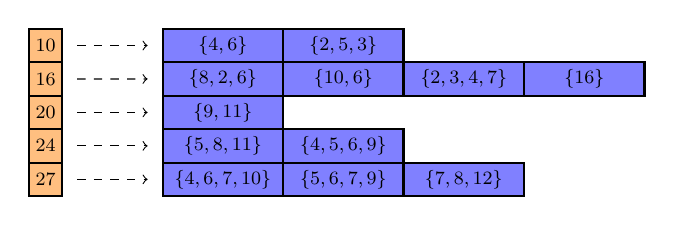
\begin{tikzpicture}
[
  scale=0.85,
  transform shape,
	key/.style={thick,fill=orange!50},
	value/.style={thick,fill=blue!50},
	other/.style={fill=yellow!10,dashed}
]

\draw (2,2) rectangle +(0.5, .5) [key] node[midway] {\textit{$10$}};
\node (10) at(2.6,2.25) {};

\draw (2,1.5) rectangle +(0.5, .5) [key] node[midway] {\textit{$16$}};
\node (16) at(2.6,1.75) {};

\draw (2,1) rectangle +(0.5, .5) [key] node[midway] {\textit{$20$}};
\node (20) at(2.6,1.25) {};

\draw (2,0.5) rectangle +(0.5, .5) [key] node[midway] {\textit{$24$}};
\node (24) at(2.6,0.75) {};

\draw (2,0) rectangle +(0.5, .5) [key] node[midway] {\textit{$27$}};
\node (27) at(2.6,0.25) {};


\node (10s) at(3.9,2.25) {};
\draw (4,2) rectangle +(1.8, .5) [value] node[midway] {\textit{$\{4,6\}$}};
\draw (5.8,2) rectangle +(1.8, .5) [value] node[midway] {\textit{$\{2,5,3\}$}};

\node (16s) at(3.9,1.75) {};
\draw (4,1.5) rectangle +(1.8, .5) [value] node[midway] {\textit{$\{8,2,6\}$}};
\draw (5.8,1.5) rectangle +(1.8, .5) [value] node[midway] {\textit{$\{10,6\}$}};
\draw (7.6,1.5) rectangle +(1.8, .5) [value] node[midway] {\textit{$\{2,3,4,7\}$}};
\draw (9.4,1.5) rectangle +(1.8, .5) [value] node[midway] {\textit{$\{16\}$}};

\node (20s) at(3.9,1.25) {};
\draw (4,1) rectangle +(1.8, .5) [value] node[midway] {\textit{$\{9,11\}$}};

\node (24s) at(3.9,0.75) {};
\draw (4,0.5) rectangle +(1.8, .5) [value] node[midway] {\textit{$\{5,8,11\}$}};
\draw (5.8,0.5) rectangle +(1.8, .5) [value] node[midway] {\textit{$\{4,5,6,9\}$}};

\node (27s) at(3.9,0.25) {};
\draw (4,0) rectangle +(1.8, .5) [value] node[midway] {\textit{$\{4,6,7,10\}$}};
\draw (5.8,0) rectangle +(1.8, .5) [value] node[midway] {\textit{$\{5,6,7,9\}$}};
\draw (7.6,0) rectangle +(1.8, .5) [value] node[midway] {\textit{$\{7,8,12\}$}};

\draw [->,thin, dashed] (10) -- (10s);
\draw [->,thin, dashed] (16) -- (16s);
\draw [->,thin, dashed] (20) -- (20s);
\draw [->,thin, dashed] (24) -- (24s);
\draw [->,thin, dashed] (27) -- (27s);

\end{tikzpicture}

  \caption{This figure shows the macrostate cache based on a hash table where the key is the sum of a macrostate and a value is a list of the macrostates.}
  \label{figMacroCache}
\end{center}
\end{figure}

\section{Implementation of the Antichains Algorithm}
The implementation of the algorithm for checking language inclusion of NFA using antichains has been done by the algorithm described in Section 
\ref{sectionAntichain}.  There were used data structures for the representation of the antichains (classes \emph{Antichain2Cv2} and \emph{Antichain1c}) which
were implemented for the modules for tree automata. 

The improvement of the antichains algorithm by using simulation is implemented too. 
This is done by parameterization of the class for checking inclusion, where one of the given parameters is a relation which is a simulation or identity.

Some optimization of this algorithm has been done during implementation and will be described in the following subsections. For further subsections we fix
NFAs $\mathcal{A}$ and $\mathcal{B}$ and consider the problem $L_{\mathcal{A}}\subseteq L_{\mathcal{B}}$.

\subsection{Ordering of an Antichain}
The antichains algorithm keeps only the minimal set of the visited product states with respect to the ordering given by $(r,R)\sqsubseteq (p,P)$
iff $p=r \wedge R \subseteq P$. The ordering $p\preceq r \wedge R\preceq^{\forall\exists}P$ is used for the optimization by simulation.
Comparing $(r,R)$ and $(p,P)$ was implemented by one parameterized function for both orderings which is possible because $p=r$ is a special case of $p\preceq r$ 
and the same holds for $R \subseteq P$ and $R\preceq^{\forall\exists}P$. But this implementation has shown as inefficient and the special implementation of
this function for each ordering alone should be more efficient because $R\subseteq P$ could be decided 
without comparing both sets element by element when the size of the macrostate $R$ is greater then size of the macrostate $P$ while in the case of
$R\preceq^{\forall\exists}P$ one element of the macrostate $P$ could simulate all elements of $R$ so the optimization cannot be used.
The ordering using simulation also needs to iterate through all visited product states to find all the elements $p$ such that $p\preceq r$ which 
is not necessary in the case of the basic version where just $p=r$ is checked.

On the other hand, the other optimization of simulation is based on the fact that if there is $p' \in P$ such that $p \preceq p'$ 
it is not needed to keep and further process the product state $(p,P)$. When one parameterized function is used for both versions of the algorithm, it 
causes unnecessary slow down because the condition is always false in the case of the basic version of the algorithm. 
Although this optimization has not been implemented yet, we suppose that the separation of the functions will be also 
efficiently used in this case.

\subsection{Using Macrostate Cache}
The antichain algorithm often checks whether $R \subseteq P$ or $R\preceq^{\forall\exists}P$ which can be both quite expensive operations and it may be
helpful to store the results of these operations. The macrostate cache has been applied for this purpose so all used macrostates (such as $R$ or $P$) 
are stored in this cache. Then it is possible to work just with the pointers to the cache which helps to efficiently 
store the relation between $R$ and $P$. For example, the pointer to $R$ is mapped to the pointer to $P$ by a hash table when there is relation between 
$R$ and $P$. There is also a hash table that maps the pointer to the macrostate $R$ to pointers to all macrostates which are not in relation with $R$.

\subsection{Ordered Antichain}
As the data structure for the $Next$ set we use an ordered antichain which prefers processing of elements with a
smaller size of the macrostate $P$ first. This optimization leads to the reduction of produced states. The optimization has been implemented 
also for checking language inclusion of NFA and it reduces the number of the produced product states too which yields a better performance.

%No further optimization for antichain algorithm are used so it is not as efficient as the algorithm based on bisimulation up to congruence and not even as the 
%tree version of this algorithm which is highly optimized. The suggestions for some optimization are given in another section \ref{Conclusion}.

\section{Translation of an NFA into an LTS}
Before computing the (maximum) simulation relation over an NFA it is necessary to convert the NFA into a LTS, sort the states of the NFA to
two or three partitions (final, non-final and the class representing initial state) and initialize the simulation relation. This is done by an algorithm where 
all transitions of the input NFA are converted to edges of the LTS and at the same time each of the processed states is sorted to the partitions according to
whether the state is final or not. If all states are final, there will be created only one partition in this part of the algorithm otherwise two partitions will
be created. After all transitions are processed, another partition representing initial states is added. Then the simulation relation is initialized
by the rules that each final state simulates other final state and each non-final simulates other non-final. A non-final one does not simulate a final one, but 
a final one simulates a non-final one.
The created partitions, LTS and initialized simulation is given to the algorithm for computing the (maximum forward) simulation. 

\section{Implementation of the Bisimulation up to Congruence Algorithm}
\label{sectionCongrImpl}
The algorithm for checking inclusion of the languages of NFA is described in Section~\ref{sectionCongr}. For computation of a congruence closure, 
which is a crucial part of the approach, we used an algorithm based on the rewriting rules (described in Section \ref{subsectionCongr}). 
This algorithm was implemented generally for checking equivalence of NFA and its optimized version for checking inclusion was implemented too 
because the main goal of this work is to achieve the best performance of the inclusion checking. In this section we will describe a few implementation
optimizations of the algorithm. 
For the rest of this section consider two NFA $\mathcal{A}=(Q_\mathcal{A},\Sigma,\delta_\mathcal{A},I_\mathcal{A},F_\mathcal{A})$ and
$\mathcal{B}=(Q_\mathcal{B},\Sigma,\delta_\mathcal{B},I_\mathcal{B},F_\mathcal{B})$.


\subsection{Exploring Product NFA}
Exploration of the product NFA $\mathcal{A}\cap\mathcal{B}$ while checking inclusion between the languages of the 
$\mathcal{A}$ and $\mathcal{B}$ could be done by 
the \emph{breadth-first search} \cite{taocp} algorithm or the \emph{depth-first search} \cite{taocp} algorithm, which
determines the order in which the states of the product NFA are explored. The use of one or another algorithm can effect the number of states that are processed. 
The difference between these two approaches is in the use of a data structure for storing of the newly generated states of $\mathcal{A}\cap\mathcal{B}$.
If the used data structure is a list then the breadth-first search is applied and if the used data structure is a stack then 
depth-first search is applied.

The VATA library module for NFA currently supports only the breadth-first search algorithm. This approach has not been chosen for any special reason or superiority
but has evolved during the implementation because the antichain algorithm also uses a list for storing of 
the newly generated states which leads to the implementation of breadth-first search.


\subsection{Using Macrostate cache}
When one checks inclusion (or equivalence) of languages of the NFA $\mathcal{A}$ and $\mathcal{B}$ there are generated states states of the 
product NFA $\mathcal{A}
\cap \mathcal{B}$ which are pairs $(X,Y)$ where $X$ is a macrostate of states of $\mathcal{A}$ and $Y$ is a macrostate of states of $\mathcal{B}$. $X$ and $Y$
are stored to the macrostates cache and it is further worked only with pointers to these macrostates in the cache.

The original algorithm does not check whether the newly generated state $(X,Y)$ has not already been visited and always checks whether $(X,Y)$ is in
the congruence closure of the relation of the visited states $R$  which is
a computationally demanding operation. Thanks to working just with pointers to macrostates it is easy to check whether the new state is already in a set of 
visited states without computing the congruence closure. This is done by a hash table which maps pointer of a macrostate $Y$ to the list of all
pointers to macrostates $X$ such that $(X,Y)\in R$. Then it is easy to check whether a newly generated state has already been processed or not. 

This technique reduces the number of the states of $\mathcal{A}\cap\mathcal{B}$ for which is necessary to compute the congruence closure which helps to
improve in the performance of the whole algorithm.

\subsection{Computing Congruence Closure for Checking Equivalence}
The computation of the congruence closure of the set of visited states of the NFA $\mathcal{A}~\cap~\mathcal{B}$ for equivalence checking using rewriting
rules as it was described in Section \ref{subsectionCongr} is a computationally demanding operation, 
so there was implemented an optimization to enhance the performance of the algorithm.

The optimization is based on the observation that when the normal forms of the macrostates $X$ and $Y$ for some relation $R$ are derived to find out whether
it holds that $(X,Y)\in c(R)$ it is not necessary to use all possible rewriting rules of $R$ and add as much states as possible to the normal form
of the macrostate. It is possible to stop the derivation of
$X{\downarrow_R}$ and $Y{\downarrow_R}$ when these sets are equal and it is also not necessary to achieve the equality between 
$X{\downarrow_R}$ and $Y{\downarrow_R}$ by applying the same rules, not even by applying the same number of rules. 
This fact makes it possible to check $X{\downarrow_R} = Y{\downarrow_R}$ on the fly and not only after the whole derivation.

This simplification leads to the implementation optimization, which is based on creating $X{\downarrow_R}$ by applying all possible rewriting rules
so that it has as many states as possible. 
When a rule is applied during the derivation of $X{\downarrow_R}$, it is mapped in a hash table to 
the form of $X{\downarrow_R}$ after application of the rule.
Then $Y{\downarrow_R}$ is derived gradually and after each step it is checked whether the current form of $Y{\downarrow_R}$ is not the same as any of the forms of
$X{\downarrow_R}$ which has been reached during its derivation. However 
comparing $Y{\downarrow_R}$ after each step to all forms of $X{\downarrow_R}$ is not efficient
and it slows down the algorithm instead of improving it. This leads to the implementation where the form of $Y{\downarrow_R}$ after applying of a rewriting rule 
is compared to the form of $X{\downarrow_R}$ after the use of the same rule. 
The second approach is not maybe so efficient because it does not detect whether 
$X{\downarrow_R}=Y{\downarrow_R}$ as early as the first one but this disadvantage is compensated by a smaller number of comparisons 
of $X{\downarrow_R}$ and $Y{\downarrow_R}$.

\subsection{Computing Congruence Closure for Inclusion Checking}
In Section \ref{congrOpt} an optimization was described that can be used when one uses the algorithm based on bisimulation up to congruence for checking 
language inclusion. The optimization is based on the fact that inclusion checking is done by checking the equivalence $\mathcal{A}\cup\mathcal{B}=\mathcal{B}$,
so for a state $(X,Y)$ it holds that $(X,Y)\in c(R)$ iff $X\subseteq Y{\downarrow_R}$ for a relation $R$ of visited states. 
This optimization was implemented in the VATA library module for NFA to achieve the best performance in checking language inclusion.

This optimization is further enhanced by the following improvements in the implementation. 
Once there is checked a generated product state $(X,Y)$ and the normal form 
$Y{\downarrow_R}$ is computed, it could be efficient to store all rewriting rules that were used during the computation because otherwise there can be
generated another product state with $Y$ in, e.g. $(Z,Y)$ and the whole computation of $Y{\downarrow_R}$ has to be done again. 

At the same time a rewriting rule can be used only in one direction ($Y\rightarrow X\cup Y$) for $(X,Y)\in R$. So when it is checked
if a newly generated product state $(P,Q)$ is in the congruence closure of $R$ it is needed just to check if $Y \subseteq Q$ to apply 
the rewriting rule $Y\rightarrow X\cup Y$. If the rewriting rule is applied, the macrostate $X$ is added to $Q{\downarrow_R}$. 
Once the rewriting rule is possible to apply we know that it is possible to apply all elements of $R$ containing $Y$ 
so it is efficient to store the relation $Y\subseteq Q$.

This principle of storing applicable rules is implemented by a hash table where a pointer to a macrostate $Q$ is mapped to
a list of pointers to the macrostates where each of this macrostates $Y$ enables to use all of the elements of the relation $R$ containing $Y$ 
for computation of $Q{\downarrow_R}$.
Notice that it is not possible to store elements of $R$ which rewriting rule is not applicable because there are added gradually
new elements to $R$ and after the application of a new rewriting rule can be usable also rule which could not be used the last time.

During the experimental evaluation it was found that this optimization is not as useful as it was expected because it does not happen very often that a single
macrostate of NFA $\mathcal{B}$ (e.g. a macrostate $Q$) is in two different states of a 
product NFA $(\mathcal{A}\cup\mathcal{B})\cap\mathcal{B}$ (e.g., $(P,Q)$
and $(O,Q)$ where $P$ and $O$ are macrostates of $\mathcal{A}\cup\mathcal{B}$) and can slow down the algorithm because of the overhead given by checking
if a normal form $Q{\downarrow_R}$ has not already been computed, so it was implemented as a special function for computing the 
normal form of a visited macrostate and a special function for computing the normal forms of macrostates which has not been already explored. 

\chapter{Experimental Evaluation}
\label{eval}
This chapter describes the experimental evaluation of the algorithms for checking inclusion based on antichains and on the bisimulation up to congruence. 

For both of the evaluations we used NFA from abstract regular model checking provided by Dr. Lukáš Holík\footnote{
Automata can be found on the web page: \url{http://www.fit.vutbr.cz/~holik/pub/ARMCautomata.tar.gz}}.  
The evaluation was done on the set of about 40 000 of pairs of NFA. 

The tests were performed on the server \emph{merlin.fit.vutbr.cz} with CentOS 64bit Linux, 2$\times$ AMD Opteron Processors (2,5 GHz, 4 cores, 12 MB cache)
and 8 GB RAM.

\section{Evaluation of Algorithm Based on Antichains}
The implementation of the antichain algorithm is compared to the VATA library implementation of the antichain algorithm for tree automata. The
algorithms for checking language inclusion of tree automata was tested in the explicit encoding using upward direction and also downward direction. 
The timeout of the computation was set to five seconds.

The comparison with the inclusion checking algorithm for tree automata in the upward direction is given in Figure \ref{fig:figPlotAac} where the whole data
set is in the left plot and the right plot is zoomed. The new implementation for NFA was faster in 98\,\% of the
test cases and in these cases was on average twice as fast. The algorithm for tree automata is faster only in 2\,\% of cases 
but in these cases it is faster sixteen times.
This acceleration of the algorithm for tree automata in some cases has not yet been analyzed and could be an object of further development.

\begin{figure}[bt]
\begin{center}
\includegraphics[scale=0.33]{fig/plot_aac_zprava.png}
\includegraphics[scale=0.33]{fig/plot_aac_step_zprava.png}
\caption{A comparison of the VATA library implementation of the antichains algorithm for tree automata in upward direction
    with the VATA library implementation of the antichains algorithm for NFA.}
\label{fig:figPlotAac}
\end{center}
\end{figure}

The comparison of the new implementation of the algorithm for NFA with the implementation for tree automata in the downward direction using the optimized cache
is given in Figure~\ref{fig:figPlotAac} 
where the left plot again shows the whole data set and the right one shows the zoom on the time interval where most of the tests belong.
The algorithm for NFA beats the algorithm tree automata in the most cases (about 93\,\%) and is about 211 times faster (all data are in Table \ref{tabAc}).

\begin{table}[bt]
\begin{center}
\parbox{.45\linewidth}{
  \begin{tabular}[scale=0.3]{ | l | r | r |}
   \hline
    & \textbf{AC UP} & \textbf{AC NFA} \\ \hline \hline
    winner & $2\,\%$ & $98\,\%$ \\ \hline
    faster & $15.91\times$ & $2.65\times$ \\ \hline
   \end{tabular}
}
   \parbox{.45\linewidth}{
  \begin{tabular}{ | l | r | r |}
   \hline
    & \textbf{AC DOWN} & \textbf{AC NFA} \\ \hline \hline
    winner & $7\,\%$ & $93\,\%$ \\ \hline
    faster & $10.78\times$ & $211.42\times$ \\ \hline
   \end{tabular}
   }
   \caption{The left table shows a comparison of the VATA library for tree automata with checking inclusion in the 
     upward direction using the antichains algorithm with the implementation of the antichains algorithm for NFA and
   the right table shows the same comparison but with for the downward direction version of the antichains algorithm for tree automata optimized
   by a cache.}
   \label{tabAac}
\end{center}
\end{table}



\begin{figure}[bt]
\begin{center}
\includegraphics[scale=0.33]{fig/plot_aca_zprava.png}
\includegraphics[scale=0.33]{fig/plot_aca_step_zprava.png}
\caption{The figure shows
 a comparison of the VATA library implementation of the antichains algorithm for tree automata in the downward direction using the cache optimization 
 with the VATA library implementation of the antichains algorithm for NFA.}
\label{fig:figPlotAca}
\end{center}
\end{figure}

\section{Evaluation of Algorithm Based on Bisimulation up to Congruence}
The evaluation of the algorithm based on bisimulation up to congruence was done with the implementation which includes all optimizations described in Section 
\ref{sectionCongrImpl}. There are two comparisons provided, the first one is with the original OCaml implementation of this algorithm \cite{popl13} 
and the second one is with the VATA library module for tree automata.

\subsection{Comparison with OCaml Implementation}
The algorithm based on bisimulation up to congruence was implemented\footnote{The implementation can be found here: \url{
http://perso.ens-lyon.fr/damien.pous/hknt/}} 
in the \emph{OCaml} language (an object-oriented implementation of the Caml language). 
This implementation provides checking of equivalence
and inclusion of languages of NFA. It also allows to choose between the breadth-first search or the depth-first search algorithm for searching the
product NFA and it is possible to use a simulation for an improvement of the performance of the algorithm.

For evaluation purposes the OCaml implementation was run with the breadth-first search (which is the only one currently implemented by the VATA library), without
simulation (which is not currently provided by the VATA library) and in the version for inclusion checking.

The comparison of the VATA library implementation and the OCaml implementation can be seen in Figure \ref{fig:figGraphOCaml}. 
The plot shows the relation between the time needed to check language inclusion and number of states of the input NFA.
The left plot shows the measurements on the whole data set and it is possible to see that the VATA library is especially faster for input automata with a lot
of states. The right plot in Figure \ref{fig:figGraphOCaml} is zoomed to the time interval where the most of the measurements belong and 
shows that in some cases the OCaml implementation is faster. In these cases only a few states were explored to 
check that the language inclusion and the VATA library was slower due to the overhead caused by its richer data structures 
(such as the macrostate cache). The plot also shows how the time needed to check inclusion grows exponentially with the number of states of NFA but 
the growth of the amount of time is much faster in the case of the OCaml implementation.

The VATA library was faster in $92.5\,\%$ of the tested cases and in these cases it was faster about 65 times. More detailed data can be found 
in Table \ref{tabOcaml}.

\begin{figure}[bt]
\begin{center}
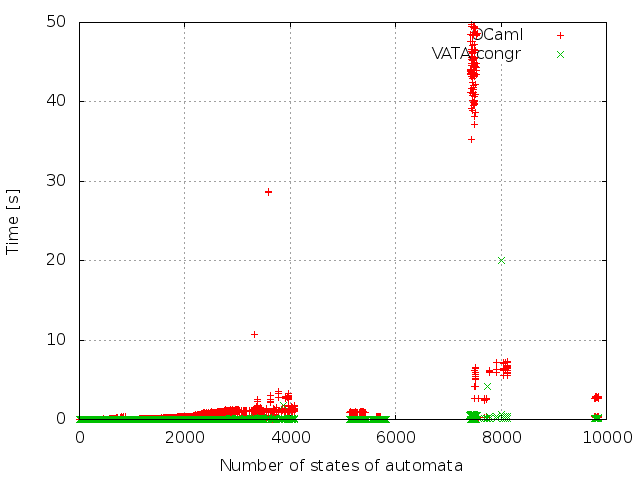
\includegraphics[scale=0.33]{fig/plot_hkc_zprava.png}
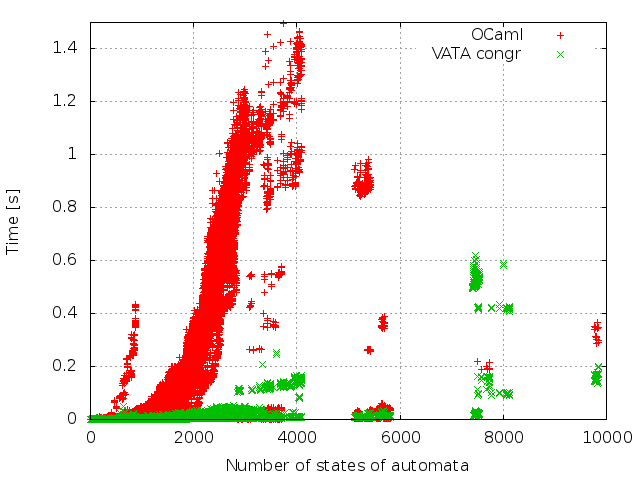
\includegraphics[scale=0.33]{fig/plot_hkc_step_zprava.png}
\caption{
Comparison of the OCaml implementation of a congruence algorithm and the VATA library implementation of the algorithm.}
\label{fig:figGraphOCaml}
\end{center}
\end{figure}

\begin{center}
\begin{table}[tb]
\begin{center}
  \begin{tabular}{ | l | r | r |}
   \hline
    & \textbf{OCaml} & \textbf{VATA} \\ \hline \hline
    winner & $7.5\,\%$ & $92.5\,\%$ \\ \hline
    faster & $6.43\times$ & $64.29\times$ \\ \hline
   \end{tabular}
   \caption{This table gives a summary of the evaluation of the performance of the OCaml implementation of a congruence algorithm and VATA library implementation 
     of the same algorithm.}
   \label{tabOcaml}
\end{center}
\end{table}
\end{center}

\subsection{Comparison with Tree Automata Implementation of VATA Library}
We have also evaluated the performance of the inclusion checking algorithm based on bisimulation up to congruence with the VATA implementation of the antichains
algorithm.
The VATA library for tree automata was used with explicit encoding and inclusion was checked in the upward and also in the downward direction. 
For downward direction an optimization based on a cache was used. The timeout for checking inclusion was set to 5 seconds.

The results of the comparison of the checking language inclusion using bisimulation up to congruence for NFA and antichains for tree automata 
are given in Figures \ref{fig:figPlotAc} and \ref{fig:figPlotCa}, where the left plots show the whole data set and the right plots are zoomed. 
The plots show the number of states of the input
automata and the time needed to check the inclusion. The new implementation for finite automata is faster in the
most (about $95\,\%$) cases but is only about twice as fast as the algorithm for upward direction. 
Checking language inclusion using downward direction is much slower than 
the congruence algorithm which is faster in $94\,\%$ of the cases  and is faster by the ratio of one hundred and sixty. The particular data about the speed-up 
of the implementation for NFA is given in Table \ref{tabAc}.

Figures \ref{fig:figPlotAc} and \ref{fig:figPlotCa} also show
focus to a time interval where the most measurements belong. The figures show that the VATA library module for tree automata was
also faster in some cases, which is caused by the fact the both approaches (antichain and bisimulation up to congruence) uses different attributes of the relation
of sets of states that are necessary to check to verify that language inclusion holds.

\begin{figure}[bt]
\begin{center}
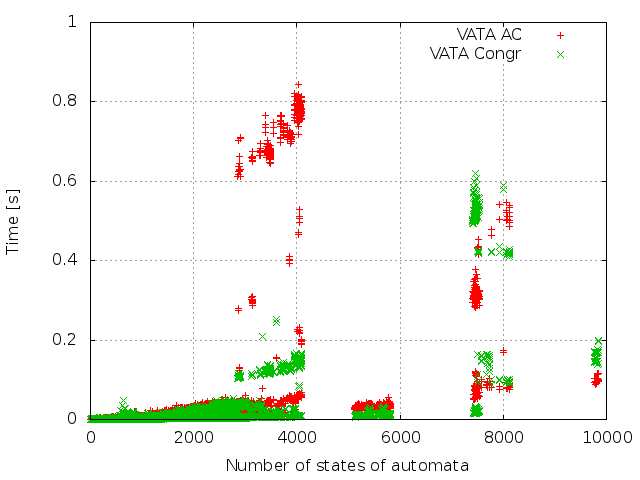
\includegraphics[scale=0.33]{fig/plot_ac_zprava.png}
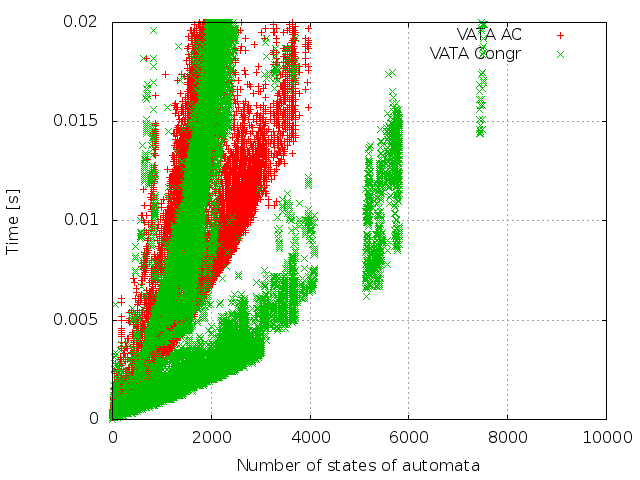
\includegraphics[scale=0.33]{fig/plot_ac_step_zprava.png}
\caption{The comparison of the VATA library implementation of the antichains algorithm for tree automata in the upward direction
    with the VATA library implementation of the congruence algorithm for NFA.}
\label{fig:figPlotAc}
\end{center}
\end{figure}

\begin{table}[bt]
\begin{center}
\parbox{.45\linewidth}{
  \begin{tabular}[scale=0.3]{ | l | r | r |}
   \hline
    & \textbf{AC UP} & \textbf{CONGR} \\ \hline \hline
    winner & $5\,\%$ & $95\,\%$ \\ \hline
    faster & $1.27\times$ & $2.34\times$ \\ \hline
   \end{tabular}
}
   \parbox{.45\linewidth}{
  \begin{tabular}{ | l | r | r |}
   \hline
    & \textbf{AC DOWN} & \textbf{CONGR} \\ \hline \hline
    winner & $6\,\%$ & $94\,\%$ \\ \hline
    faster & $1.90\times$ & $160.34\times$ \\ \hline
   \end{tabular}
   }
   \caption{The left table shows a comparison of the VATA library for tree automata with checking inclusion upward using the antichains algorithm with
       the implementation of the algorithm based on bisimulation up to congruence, and
   the right table shows the same comparison but for the downward version of the antichains algorithm optimized by cache.}
   \label{tabAc}
\end{center}
\end{table}

\begin{figure}[t]
\begin{center}
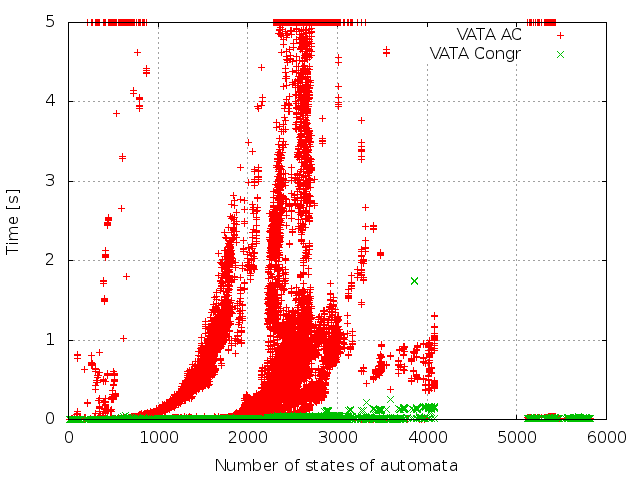
\includegraphics[scale=0.33]{fig/plot_ca_zprava.png}
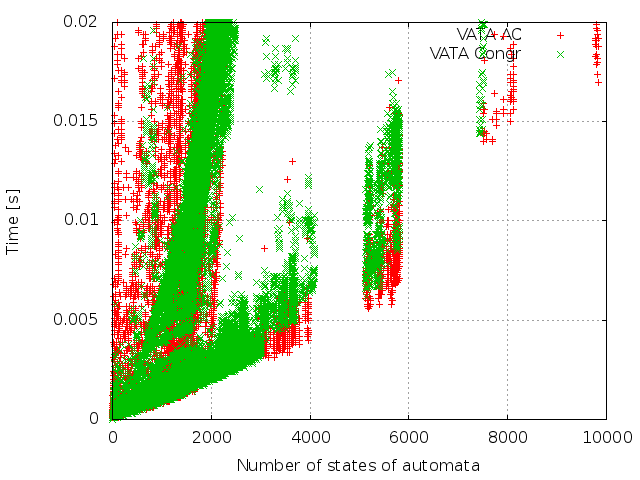
\includegraphics[scale=0.33]{fig/plot_ca_step_zprava.png}
\caption{The figure shows a
 comparison of the VATA library implementation of the antichains algorithm for tree automata in the downward direction using the cache optimization 
 with the VATA library implementation of the congruence algorithm for NFA.}
\label{fig:figPlotCa}
\end{center}
\end{figure}

\section{Comparison of the Algorithms for NFA}
Finally, both newly implemented algorithms for NFA, the one based on the antichains and the one based on the bisimulation up to congruence, will be compared.
Both algorithms were used in their optimized versions.
The comparison is shown in Figure \ref{fig:figPlotNFA}.
As you can see, the results of the evaluations of both algorithms are very similar and the differences in their performance are very small. 
The results are summarized in Table \ref{tabNFA}. The antichain algorithm beats the congruence algorithm in 75\,\% of
the tested cases. On the other hand, the congruence algorithm is nearly four times faster in its winning cases than the antichains algorithm which is
only 1.5 times faster in its winning cases. 
It is important to notice that the results depend on the chosen test set because both algorithms use different attributes
of the set of explored states of the NFA while checking language inclusion.

\begin{figure}[bt]
\begin{center}
\includegraphics[scale=0.33]{fig/plot_nfa_ac_zprava.png}
\includegraphics[scale=0.33]{fig/plot_nfa_congr_zprava.png}
\caption{The comparison of the VATA library implementation of the antichains algorithm for NFA (the left plot)
    with the VATA library implementation of the congruence algorithm for NFA (the right plot).}
\label{fig:figPlotNFA}
\end{center}
\end{figure}

\begin{table}[bt]
\begin{center}
\parbox{.45\linewidth}{
  \begin{tabular}[scale=0.3]{ | l | r | r |}
   \hline
    & \textbf{AC} & \textbf{CONGR} \\ \hline \hline
    winner & $76\%$ & $24\%$ \\ \hline
    faster & $1.58\times$ & $3.74\times$ \\ \hline
   \end{tabular}
}
   \caption{This table shows the result of a comparison of the congruence algorithm and the antichain algorithm for NFA.}
   \label{tabNFA}
\end{center}
\end{table}
\hfill

\chapter{Conclusion}
\label{concl}
The main goal of this thesis was to create an extension of the VATA library for nondeterministic finite automata 
that are often used in formal verification (e.g., in model checking of safety temporal properties or in 
abstract regular model checking) which is the target area of the use of the library. The extension of the library supports
basic operations like union, intersection, removing useless or unreachable states etc., but the main aim of this work was to provide
an efficient implementation of state-of-the-art algorithms for checking language inclusion of nondeterministic finite automata.

The data structures for the explicit encoding for representation of finite automata has been designed
and implemented by modification and optimization of the data structures for tree automata already presented in the VATA library. 
The original VATA library has been analyzed to determine
which modules can be reused for the new extension and also to efficiently integrate the new extension.

To achieve the best performance for language inclusion checking we use state-of-the-art algorithms, based on so-called antichains and so-called bisimulation
up to congruence. The antichains algorithm was implemented in its default version and also in an optimized version which uses simulation over a finite automaton. 
The bisimulation up to congruence algorithm is implemented in its general version (for checking language equivalence of NFA) and also in
the version specialized to checking inclusion. %, which brings better performance. 
The other improvement of this algorithm is achieved by optimization of implementation.

An evaluation comparing the performance of our implementations and other implementations of checking language inclusion over NFA has been performed.
Our implementation beats the other tested implementations in over 90\,\% of the tested cases. It is faster about 100 times than the OCaml implementation of the
algorithm for congruence closure and twice as fast as the algorithm over tree automata.

A more detailed analysis of the cases where the algorithm for checking language inclusion over tree automata significantly 
beats the implementation specialized on NFA could be done for further optimization. 
For the bisimulation up to congruence algorithm it is possible to implement a version of the algorithm 
which uses simulation for pruning out some other states which are not necessary to explore. The simulation has already been implemented for antichains 
algorithm but it has not been evaluated and optimized which could bring another improvement in performance. 
Yet another interesting direction is to find suitable use cases of DFA for various task and evaluate whether they can improved by the use of NFA, in
particular using the extension of the VATA library developed in this work.
